\documentclass[12pt, a4paper, oneside]{thesis}
\usepackage{tgheros}
\usepackage[utf8]{inputenc}
\usepackage{kpfonts}
\usepackage[T1]{fontenc}
\usepackage[francais]{babel}
\usepackage{graphicx}
\usepackage{lmodern}
\usepackage{datetime}
\usepackage{fancyhdr}
\usepackage{listings}
\usepackage{xcolor}
\usepackage{pgf-umlsd}
\usepackage{pdflscape}
\usepackage{hyperref}
\usepackage{pdfpages}
\usepackage{lastpage}

\usepackage{geometry}
\geometry{hmargin=2.5cm,vmargin=1.5cm}

\newcommand{\subsubsubsection}[1]{\paragraph{#1}\mbox{}\par}
\setcounter{secnumdepth}{4} % Allows numbering up to four levels


\newdateformat{mydate}{\THEDAY\space\monthname[\THEMONTH]\space\THEYEAR}

\lstset{
  basicstyle=\footnotesize\ttfamily,
  commentstyle=\color{gray},
  keywordstyle=\color{blue},
  stringstyle=\color{purple},
  numbers=left,
  numbersep=5pt,
  frame=single,
  rulecolor=\color{black},
  tabsize=2,
  captionpos=b,
  breaklines=true,
  breakatwhitespace=true,
  showspaces=false,
  showstringspaces=false,
  showtabs=false,
  morecomment=[l]{\#}
}

\lstdefinelanguage{JavaScript}{
  morekeywords=[1]{break, continue, delete, else, for, function, if, in,
    new, return, this, typeof, var, void, while, with},
  % Literals, primitive types, and reference types.
  morekeywords=[2]{false, null, true, boolean, number, undefined,
    Array, Boolean, Date, Math, Number, String, Object},
  % Built-ins.
  morekeywords=[3]{eval, parseInt, parseFloat, escape, unescape},
  sensitive,
  morecomment=[s]{/*}{*/},
  morecomment=[l]//,
  morecomment=[s]{/**}{*/}, % JavaDoc style comments
  morestring=[b]',
  morestring=[b]"
}[keywords, comments, strings]

\renewcommand{\lstlistingname}{}
\renewcommand{\thesection}{\arabic{section}}

\usepackage{fancyhdr}

\fancypagestyle{plain}{
  \fancyhf{} % clear all header and footer fields for the first page
  \renewcommand{\headrulewidth}{0pt}
  \renewcommand{\footrulewidth}{0pt}
}

\pagestyle{fancy}
\fancyhf{} % clear all header and footer fields
\fancyhead{} % efface le contenu du haut de page
\fancyfoot[L]{Rapport SAE5.ROM.03} % Gauche du pied de page
\fancyfoot[C]{\thepage/59} % Numéro de page / Total de pages au centre du pied de page
\fancyfoot[R]{\href{https://portfolio.louispluviose.fr}{PLUVIOSE} - \href{https://karap.fr}{KARAPETYAN}} % Droite du pied de page
\renewcommand{\headrulewidth}{0pt} % Pas de ligne en haut de page
\renewcommand{\footrulewidth}{0pt} % Pas de ligne en bas de page

\newcommand{\newthreadShift}[4][gray!30]{
  \newinst[#4]{#2}{#3}
  \stepcounter{threadnum}
  \node[below of=inst\theinstnum,node distance=0.8cm] (thread\thethreadnum) {};
  \tikzstyle{threadcolor\thethreadnum}=[fill=#1]
  \tikzstyle{instcolor#2}=[fill=#1]
}

\usepackage{titlesec}

% Aligner les titres à gauche
\titleformat{\section}
  {\normalfont\Large\bfseries}{\thesection}{1em}{}
\titleformat{\subsection}
  {\normalfont\large\bfseries}{\thesubsection}{1em}{}
\titleformat{\subsubsection}
  {\normalfont\normalsize\bfseries}{\thesubsubsection}{1em}{}

% Justifier le texte des titres si nécessaire
\titlespacing*{\section}
  {0pt}{3.5ex plus 1ex minus .2ex}{2.3ex plus .2ex}
\titlespacing*{\subsection}
  {0pt}{3.25ex plus 1ex minus .2ex}{1.5ex plus .2ex}
\titlespacing*{\subsubsection}
  {0pt}{3.25ex plus 1ex minus .2ex}{1.5ex plus .2ex}

\begin{document}

\author{\href{https://portfolio.louispluviose.fr}{PLUVIOSE Louis} - \href{https://karap.fr}{KARAPETYAN Mikhail}}

\begin{center}
{\LARGE \textbf{Rapport SAE5.ROM.03}}

\vspace{1cm}

{\Large {\href{https://portfolio.louispluviose.fr}{PLUVIOSE Louis} - \href{https://karap.fr}{KARAPETYAN Mikhail}}}

\vspace{1cm}

{\LARGE \textbf{Application de communication WebRTC}}

\vspace{2cm}


\includegraphics[width=7.5cm]{images/logo-iut-colmar.jpg}

\vspace{0.5cm}


\includegraphics[width=7.5cm]{images/logo-but-rt.png}

\vspace{2cm}

\textbf{Sujet proposé par : Monsieur Philippe Hensel} \\

\vspace{1cm}

Université de Haute-Alsace \\
Institut Universitaire de Technologie de Colmar \\
Département Réseaux et Télécommunications \\

\vspace{3cm}

{\large \mydate\today}

\end{center}

\newpage

\tableofcontents

\lstlistoflistings

\listoffigures

\newpage

\section{Introduction}

Dans un monde de plus en plus connecté, la communication en temps réel via Internet est devenue une nécessité cruciale, tant pour les interactions personnelles que professionnelles. Notre projet pour la SAE5.ROM.03, s'inscrit dans cette dynamique en offrant une solution de communication basée sur la technologie WebRTC (Web Real-Time Communication). Nous avons voulu via ce projet nous lancer un défi : celui de permettre des échanges audio et vidéo en temps réel directement depuis le navigateur web, sans nécessité de télécharger des logiciels tiers ou de créer des comptes d'utilisateur.\\

La technologie WebRTC, un standard ouvert et gratuit, permet de réaliser des appels vidéo et audio de haute qualité avec une faible latence, garantissant ainsi une communication fluide et efficace. Notre application SAE5.ROM.03 est conçue pour être intuitive et facilement accessible, offrant une interface utilisateur élégante et des fonctionnalités adaptées à divers contextes, que ce soit pour des réunions, des sessions de travail collaboratif, ou des conversations personnelles.\\

L'accent est mis sur la facilité d'utilisation. Les utilisateurs peuvent créer et rejoindre des salles de conférence virtuelles en quelques clics, tout en bénéficiant d'une connexion fiable. De plus, l'application prend en charge plusieurs participants.\\

Une démonstration de l'application est disponible à l'adresse suivante : \url{https://webrtc.louispluviose.fr/}
\newpage

\section{Diagrammes de séquence}

\subsection{Connexion à la salle de réunion}

\begin{sequencediagram}
  \newthread{c1}{Client 1}
  \newinst[3]{s}{Server}
  \newthreadShift{c2}{Client 2}{3cm}

  % Connexion du client 1 et jointure à une salle
  \begin{sdblock}{Join Room}{Client 1 rejoins une salle de vidéo conférence}
    \begin{call}{c1}{join(roomId)}{s}{}
    \end{call}
  \end{sdblock}

  % Connexion du client 2 à la même salle
  \begin{sdblock}{Join Room}{Client 2 rejoins une salle de vidéo conférence}
    \begin{call}{c2}{join(roomId)}{s}{}
    \end{call}

  \end{sdblock}

  % Le serveur notifie le Client 2
  \begin{messcall}{s}{new\_peer}{c2}
  \end{messcall}

  % Le serveur notifie le Client 2
  \begin{messcall}{s}{new\_peer}{c1}
  \end{messcall}
\end{sequencediagram}

\newpage

\subsection{Connection WebRTC}

\begin{sequencediagram}
  \newthread{c1}{Client 1}
  \newinst[3]{s}{Server}
  \newthreadShift{c2}{Client 2}{3cm}

  \begin{sdblock}{WebRTC Connection}{Échange d'offres et de réponses pour la diffusion de vidéos}
    \begin{call}{c1}{createOffer()}{c1}{offer}
    \end{call}
    \begin{call}{c1}{setLocalDescription(offer)}{c1}{}
    \end{call}
    \begin{messcall}{c1}{offer}{s}
    \end{messcall}
    \begin{messcall}{s}{offer}{c2}
    \end{messcall}

    % Client 2 crée une réponse
    \begin{call}{c2}{createAnswer()}{c2}{answer}
    \end{call}
    \begin{call}{c2}{setLocalDescription(answer)}{c2}{}
    \end{call}
    \begin{messcall}{c2}{answer}{s}
    \end{messcall}
    \begin{messcall}{s}{answer}{c1}
    \end{messcall}
  \end{sdblock}
\end{sequencediagram}

\newpage

\subsection{Échanges de candidats ICE}

\begin{sequencediagram}
  \newthread{c1}{Client 1}
  \newinst[3]{s}{Server}
  \newthreadShift{c2}{Client 2}{3cm}

  % ICE Candidate exchange
  \begin{sdblock}{ICE Candidate Exchange}{}
    \begin{messcall}{c1}{ICE Candidate}{s}
    \end{messcall}
    \begin{messcall}{s}{ICE Candidate}{c2}
    \end{messcall}
    \begin{messcall}{c2}{ICE Candidate}{s}
    \end{messcall}
    \begin{messcall}{s}{ICE Candidate}{c1}
    \end{messcall}
  \end{sdblock}

  % Streaming video
  \begin{messcall}{c1}{stream video/audio}{c2}
  \end{messcall}
  \begin{messcall}{c2}{stream video/audio}{c1}
  \end{messcall}

  % Hang up or disconnect
  \begin{messcall}{c1}{disconnect}{s}
  \end{messcall}
  \begin{messcall}{s}{disconnect}{c2}
  \end{messcall}
\end{sequencediagram}

\newpage

\subsection{fonctionnalités supplémentaires}

\begin{sequencediagram}

  \newthread{c1}{Client 1}
  \newinst[3]{s}{Server}
  \newthreadShift{c2}{Client 2}{3cm}
  % Additional interactions based on the given code
  \begin{sdblock}{Additional Interactions}{}
    \begin{messcall}{c1}{toggleMicrophone}{c1}
    \end{messcall}
    \begin{messcall}{c1}{toggleCamera}{c1}
    \end{messcall}
    \begin{messcall}{c2}{toggleMicrophone}{c2}
    \end{messcall}
    \begin{messcall}{c2}{toggleCamera}{c2}
    \end{messcall}
  \end{sdblock}

\end{sequencediagram}

\newpage

\section{Utilisation de l'application}

\subsection{Les Réunions}

La page Réunion est spécialement conçue pour orchestrer des réunions virtuelles en temps réel en utilisant une application WebRTC. Découvrez comment les utilisateurs peuvent tirer parti de cette fonctionnalité immersive:

\subsection*{Entrer dans une salle de réunion:}
\begin{itemize}
  \item Saisir le numéro de la salle dans le champ prévu. (Le numéro de la salle peut être choisi librement sans aucune restriction.)
  \item Cliquer sur "Rejoindre la salle de réunion" pour établir la connexion.
  \item Lors de la première connexion, l'utilisateur est invité à autoriser l'accès à la caméra et au microphone en fonction du navigateur utilisé.
  \item Cliquer sur "Autoriser" pour permettre l'accès à la caméra et au microphone.
  \item L'utilisateur est désormais connecté à la salle de réunion, prêt à participer de manière interactive.
\end{itemize}

\subsection*{Vidéoconférence:}
\begin{itemize}
  \item L'interface vidéo offre une vue complète avec la vidéo locale de l'utilisateur et celles des autres participants.
  \item Après s'être connecté à la salle de réunion, l'utilisateur peut visualiser sa propre vidéo ainsi que celles des autres participants, créant une expérience immersive.
  \item La plateforme prend en charge jusqu'à trois vidéos distantes simultanées, favorisant une collaboration fluide.
\end{itemize}

\subsection*{Gestion des actions:}
\begin{itemize}
  \item Bouton "Abandonner l'appel" pour quitter la réunion avec une sortie aisée.
  \item Bouton "Activer/Désactiver le microphone" pour contrôler la diffusion audio.
  \item Bouton "Activer/Désactiver la caméra" pour gérer la visibilité vidéo selon les besoins de l'utilisateur.
\end{itemize}

\newpage

\subsection{La Messagerie en Temps Réel}

La page Messagerie est dédiée à la communication textuelle en temps réel, offrant une plateforme de discussion instantanée. Découvrez comment les utilisateurs peuvent exploiter cette fonctionnalité:

\subsection*{Saisie d'informations | Envoi de messages:}
\begin{itemize}
  \item Entrer le nom d'utilisateur dans le champ prévu. (Ce nom sera affiché dans les messages, permettant une identification claire pour les autres participants.)
  \item Saisir le message dans le champ dédié, permettant une expression libre et instantanée.
  \item Cliquer sur le bouton "Envoyer" pour partager le message avec l'ensemble des participants, favorisant l'interaction dynamique.
\end{itemize}

\subsection*{Affichage des messages:}
\begin{itemize}
  \item Les messages s'affichent clairement avec le nom de l'expéditeur et le contenu du message.
  \item Un style distinct est appliqué aux messages de l'utilisateur actuel, facilitant une identification rapide.
  \item Les messages sont présentés dans l'ordre chronologique, offrant une vue contextuelle de la conversation.
\end{itemize}


\newpage

\section{Fonctionnement de l'application de réunion}

Le code relatif à l'application est disponnible sur GitHub à l'adresse suivante \href{https://github.com/mIKIII77/SAE5.ROM.03}: et en annexe de ce document.

\subsection{DOM Elements}

\begin{itemize}
  \item \verb|const roomSelectionContainer = document.getElementById('room-selection-container');| : Cette ligne crée une constante roomSelectionContainer et lui attribue l'élément DOM (Document Object Model) dont l'identifiant (ID) est 'room-selection-container'. L'élément récupéré est un conteneur dans le code HTML où les utilisateurs peuvent sélectionner ou entrer des informations pour rejoindre une salle de chat vidéo.
  \item \verb|const roomInput = document.getElementById('room-input');| : cette ligne crée une constante roomInput qui référence l'élément DOM avec l'ID 'room-input'. Cet élément est un champ de saisie où les utilisateurs peuvent entrer le nom ou le numéro de la salle qu'ils souhaitent rejoindre.
  \item \verb|const connectButton = document.getElementById('connect-button');| :  Cette ligne crée une constante connectButton qui référence un élément DOM, probablement un bouton, avec l'ID 'connect-button'. Ce bouton est utilisé pour initier la connexion à la salle de chat vidéo après que l'utilisateur a saisi les informations nécessaires.
  \item \verb|const videoChatContainer = document.getElementById('video-chat-container');| : videoChatContainer est défini comme référençant l'élément DOM avec l'ID 'video-chat-container'. Cet élément est le conteneur principal où la vidéo du chat et d'autres éléments d'interface liés au chat vidéo seront affichés une fois la connexion établie.
  \item \verb|const localVideoComponent = document.getElementById('local-video');| :  cette ligne définit localVideoComponent comme une référence à l'élément DOM avec l'ID 'local-video'. Cet élément est utilisé pour afficher la vidéo locale de l'utilisateur, c'est-à-dire, la vidéo capturée par la caméra de l'appareil de l'utilisateur.
\end{itemize}

\vspace{0.5cm}

En résumé, ce code initialise des constantes pour référencer divers éléments d'une interface de chat vidéo, probablement définis dans le HTML. Ces références sont ensuite utilisées dans d'autres parties du code JavaScript pour gérer la logique de connexion à une salle de chat vidéo et pour contrôler l'affichage et la mise à jour de l'interface utilisateur en fonction des actions de l'utilisateur.
\newpage

\subsection{Variables}

\begin{itemize}
  \item \verb|const socket = io();| : Cette ligne crée une variable socket en utilisant io(), qui est une fonction de la bibliothèque Socket.IO. Socket.IO est une bibliothèque JavaScript pour les applications web en temps réel qui permet une communication bidirectionnelle en temps réel entre les navigateurs web et les serveurs. socket serait utilisé pour gérer les communications en temps réel, comme envoyer et recevoir des signaux pour établir des connexions vidéo.
  \item \verb|const mediaConstraints = { audio: true, video: { width: 1280, height: 720 } };| : Cette ligne définit les contraintes pour les médias qui seront utilisés dans la communication. Ici, audio: true signifie que l'audio sera activé, et video: { width: 1280, height: 720 } définit la résolution de la vidéo à 1280x720 pixels.
  \item \verb|let localStream;| : Déclaration d'une variable localStream. Cette variable sera utilisée plus tard pour stocker le flux de médias local (audio et vidéo) de l'utilisateur.
  \item \verb|let roomId;| : Déclaration d'une variable roomId qui sera utilisée pour stocker l'identifiant de la salle de chat vidéo à laquelle l'utilisateur se connecte.
  \item \verb|let peerConnections = {};| : Cette ligne initialise un objet JavaScript peerConnections comme un dictionnaire vide. Ce dictionnaire sera utilisé pour stocker toutes les connexions peer-to-peer (P2P) établies durant la session de chat vidéo. Chaque connexion P2P représente une connexion directe à un autre utilisateur dans le chat vidéo.
  \item \verb|const iceServers = { ... };| : Cette partie définit un objet iceServers qui contient la configuration des serveurs ICE (Interactive Connectivity Establishment). ICE est utilisé dans les applications WebRTC pour faciliter la connexion entre les pairs à travers différents types de réseaux et de pare-feu/NAT.
  \subitem À l'intérieur de cet objet, deux types de serveurs sont configurés :
  \subsubitem Un serveur STUN (stun:stun.l.google.com:19302), qui aide à découvrir l'adresse IP publique de l'utilisateur.
  \subsubitem Un serveur TURN (turn:relay1.expressturn.com:3478 avec un nom d'utilisateur et un mot de passe), qui est utilisé pour relayer le trafic si une connexion P2P directe n'est pas possible.
\end{itemize}

\vspace{0.5cm}

En résumé, Ce code initialise des variables clés pour la gestion de la communication en temps réel et du streaming vidéo. Il crée une connexion Socket.IO, définit les contraintes des médias (audio et vidéo), prépare des variables pour stocker le flux local et l'ID de la salle, et configure un dictionnaire pour gérer les connexions peer-to-peer. Il définit également des serveurs ICE pour aider à la connectivité réseau dans WebRTC.

\newpage

\subsection{Button Listeners}

\begin{itemize}
  \item \verb|connectButton.addEventListener('click', () => { joinRoom(roomInput.value); });| : Cette ligne attache un écouteur d'événement au bouton connectButton. Lorsque ce bouton est cliqué, la fonction anonyme déclenche l'appel de la fonction joinRoom avec la valeur actuelle de l'élément roomInput comme argument. joinRoom est une fonction qui gère la logique pour rejoindre une salle de chat vidéo spécifique basée sur l'identifiant de la salle fourni.
  \item \verb|Déclarations des boutons hangUpButton, toggleMicButton et toggleCameraButton| : Ces lignes récupèrent des références à trois boutons de l'interface utilisateur : un pour raccrocher l'appel, un pour activer/désactiver le microphone, et un pour activer/désactiver la caméra.
  \item \verb|Ajout de gestionnaires d'événements pour les boutons| : 
  \subitem \verb|hangUpButton.addEventListener('click', hangUpCall);| : ajoute un gestionnaire d'événement pour gérer l'action de raccrocher l'appel.
  \subitem \verb|toggleMicButton.addEventListener('click', toggleMicrophone);| : ajoute un gestionnaire pour activer ou désactiver le microphone.
  \subitem \verb|toggleCameraButton.addEventListener('click', toggleCamera);| : ajoute un gestionnaire pour activer ou désactiver la caméra.
  \item \verb|let isRoomCreator = false;| : Cette ligne déclare une variable isRoomCreator et l'initialise à false. Cette variable est utilisée pour suivre si l'utilisateur actuel est celui qui a créé la salle de chat vidéo. Cela peut affecter la logique de l'application, comme qui a le droit de contrôler certaines fonctionnalités de la salle ou d'inviter d'autres utilisateurs.
\end{itemize}
\vspace{0.5cm}

En résumé, Dans cet extrait, des écouteurs d'événements sont ajoutés à divers boutons de l'interface utilisateur. Ces boutons permettent de rejoindre une salle de chat vidéo, de raccrocher l'appel, d'activer/désactiver le microphone, et d'activer/désactiver la caméra. Une variable isRoomCreator est également définie pour suivre si l'utilisateur est le créateur de la salle.

\newpage

\subsection{Socket Event Callbacks}

\begin{itemize}
  \item \verb|socket.on('room_created', async () => { ... });| : Quand le serveur envoie un message room\_created, cela signifie que l'utilisateur a créé une nouvelle salle. Le flux vidéo local est configuré et isRoomCreator est défini sur true.
  \item \verb|socket.on('room_joined', async () => { ... });| : Ce gestionnaire réagit au message room\_joined, indiquant que l'utilisateur a rejoint une salle existante. Le flux local est configuré, isRoomCreator est défini sur false, et un message start\_call est émis pour commencer l'appel.
  \item \verb|socket.on('full_room', () => { ... });| : Réagit au message full\_room, indiquant que la salle que l'utilisateur tente de rejoindre est pleine. Affiche une alerte pour informer l'utilisateur.
  \item \verb|socket.on('start_call', async () => { ... });| : Lors de la réception d'un message start\_call, si l'utilisateur est le créateur de la salle, il initie les connexions Peer-to-Peer (P2P) avec les autres participants.
  \item \verb|socket.on('webrtc_offer', async (data) => { ... });| : Gère les offres WebRTC reçues d'autres pairs. Si le flux local n'est pas encore configuré, il le fait, puis traite l'offre WebRTC.
  \item \verb|socket.on('webrtc_answer', (data) => { ... });| : Gère les réponses WebRTC reçues en réponse à une offre envoyée précédemment.
  \item \verb|socket.on('webrtc_ice_candidate', (data) => { ... });| : Gère les messages de candidats ICE, qui sont des informations nécessaires pour établir la connectivité réseau dans WebRTC.  
  \item \verb|socket.on('new_peer', async (peerId) => { ... });| : Réagit à un message indiquant qu'un nouveau pair a rejoint la salle, et initie la configuration d'une connexion P2P avec ce nouveau pair. 
\end{itemize}

\vspace{0.5cm}

En résumé, cet extrait définit plusieurs gestionnaires d'événements pour gérer les communications via Socket.IO dans notre application de chat vidéo WebRTC. Ces événements incluent la création et la jonction à des salles, la gestion de salles pleines, le démarrage d'appels, et la gestion des offres, réponses, et candidats ICE de WebRTC, ainsi que la gestion de l'arrivée de nouveaux pairs.

\newpage

\subsection{Fonctions Principales}

\begin{enumerate}
  \item \verb|joinRoom(room)|
  \begin{itemize}
    \item But : Afficher l'interface de la conférence vidéo.
    \item Fonctionnement : Masque le conteneur de sélection de salle et affiche le conteneur de chat vidéo. Masque également le texte d'attente.
  \end{itemize}
  \item \verb|showVideoConference()|
  \begin{itemize}
    \item But : Afficher l'interface de la conférence vidéo.
    \item Fonctionnement : Masque le conteneur de sélection de salle et affiche le conteneur de chat vidéo. Masque également le texte d'attente.
  \end{itemize}
  \item \verb|setLocalStream(mediaConstraints)|
  \begin{itemize}
    \item But : Configurer le flux de médias local.
    \item Fonctionnement : Obtient le flux multimédia local selon les contraintes fournies et l'affecte à l'élément vidéo local.
  \end{itemize}
  \item \verb|handleNewPeer(peerId)|
  \begin{itemize}
    \item But : Gérer l'arrivée d'un nouveau pair.
    \item Fonctionnement : Crée une connexion peer-to-peer avec le nouveau pair, ajoute le flux local à cette connexion, crée une offre WebRTC et l'envoie au pair via le socket.
  \end{itemize}
  \item \verb|setupPeerConnection(peerId, isInitiator)|
  \begin{itemize}
    \item But : Configurer une connexion peer-to-peer.
    \item Fonctionnement : Crée une nouvelle connexion WebRTC avec les serveurs ICE configurés, ajoute des gestionnaires pour les événements track et icecandidate, et si l'utilisateur est l'initiateur, crée et envoie une offre WebRTC.
  \end{itemize}
  \item \verb|addRemoteStream(event, peerId)|
  \begin{itemize}
    \item But : Ajouter un flux distant à l'interface utilisateur.
    \item Fonctionnement : Crée un nouvel élément vidéo pour le flux distant ou utilise un élément existant, puis associe le flux distant à cet élément vidéo.
  \end{itemize}
  \item \verb|handleIceEvent(event, peerId)|
  \begin{itemize}
    \item But : Traiter une offre WebRTC reçue.
    \item Fonctionnement : Configure la description distante, gère les candidats ICE mis en cache, crée une réponse et l'envoie au pair.
  \end{itemize}
  \item \verb|handleAnswer(data)|
  \begin{itemize}
    \item But : Traiter une réponse WebRTC reçue.
    \item Fonctionnement : Met à jour la description distante de la connexion peer-to-peer.
  \end{itemize}
  \item \verb|handleIceCandidate(data)|
  \begin{itemize}
    \item But : Gérer les candidats ICE reçus.
    \item Fonctionnement : Ajoute les candidats ICE à la connexion peer-to-peer correspondante.
  \end{itemize}
  \item \verb|hangUpCall()|
  \begin{itemize}
    \item But : Terminer l'appel en cours.
    \item Fonctionnement : Ferme toutes les connexions peer-to-peer, arrête le flux local et nettoie l'interface utilisateur.
  \end{itemize}
  \item \verb|toggleMicrophone()|
  \begin{itemize}
    \item But : Activer ou désactiver le microphone.
    \item Fonctionnement : Bascule l'état d'activation de la piste audio du flux local.
  \end{itemize}
  \item \verb|toggleCamera()|
  \begin{itemize}
    \item But : Activer ou désactiver la caméra.
    \item Fonctionnement : Bascule l'état d'activation de la piste vidéo du flux local.
  \end{itemize}
\end{enumerate}

\newpage

\section{Fonctionnement de l'application de messagerie}
\subsection{Initialisation et Connexion Socket.IO}

\begin{itemize}
  \item \verb|Écouteur d'événement 'DOMContentLoaded| : Le code s'exécute une fois que le contenu de la page est complètement chargé.
  \item \verb|Création d'une socket : const socket = io();| : initialise une connexion Socket.IO avec le serveur.
  \item \verb|Génération d'un identifiant utilisateur : const userId = Date.now().toString();| : crée un identifiant unique pour chaque utilisateur en utilisant le timestamp actuel.
  \item \verb|Connexion à Socket.IO| : L'écouteur socket.on('connect', ...) est déclenché lorsque le client est connecté au serveur Socket.IO.
\end{itemize}
\vspace{0.5cm}

\subsection{Éléments de l'Interface Utilisateur}

\begin{itemize}
  \item \verb|Sélection des éléments DOM | : Les éléments pour le bouton d'envoi, la zone d'affichage des messages, le champ de saisie du nom d'utilisateur et le champ de saisie du message sont récupérés.
\end{itemize}
\vspace{0.5cm}

\subsection{Envoi de Messages}

\begin{itemize}
  \item \verb|Écouteur d'événement pour le bouton d'envoi| : Lorsque le bouton d'envoi est cliqué, le nom d'utilisateur et le message sont récupérés.
  \item \verb|Validation et envoi du message| : Si le message n'est pas vide, il est envoyé au serveur via socket.emit('chat\_message', { userId, username, message }).
  \item \verb|Réinitialisation du champ de saisie du message| : Le champ de saisie du message est vidé après l'envoi du message.
\end{itemize}
\vspace{0.5cm}

\subsection{Réception et Affichage de Messages}

\begin{itemize}
  \item \verb|Écouteur d'événement pour 'chat_message'| : Lorsqu'un message est reçu du serveur, il déclenche l'exécution du code suivant :
  \item \verb|Création de conteneurs pour le message| : Un div pour contenir le message et un autre div pour le texte du message sont créés et stylisés.
  \item \verb|Identification de l'expéditeur| : Un élément strong est utilisé pour afficher le nom de l'expéditeur en gras. Il affiche "Vous" si l'identifiant de l'expéditeur correspond à celui de l'utilisateur actuel, sinon le nom d'utilisateur de l'expéditeur.
  \item \verb|Ajout du message| : Le texte du message est ajouté après le nom de l'expéditeur.
  \item \verb|Stylisation basée sur l'expéditeur| : Les styles sont appliqués différemment pour distinguer visuellement les messages envoyés par l'utilisateur actuel de ceux des autres utilisateurs.
  \item \verb|Ajout du message à l'interface utilisateur| : Le conteneur de message est ajouté à messagesDiv.
  \item \verb|Défilement automatique| : L'affichage des messages défile automatiquement vers le bas pour montrer les nouveaux messages.
\end{itemize}

\vspace{0.5cm}

\subsection{Résumé}

Ce script crée un client de chat en temps réel. Lorsqu'un utilisateur envoie un message, il est transmis au serveur via Socket.IO, puis distribué à tous les clients connectés. Les messages entrants sont affichés dans l'interface utilisateur avec une distinction entre les messages de l'utilisateur actuel et ceux des autres utilisateurs. Ce script démontre une utilisation typique de Socket.IO pour une application de chat interactive.

\newpage

\section{Fonctionnement du serveur de l'application}
\subsection{Initialisation d'Express et Configuration SSR}

\begin{itemize}
  \item \verb|Importation des modules nécessaires| : Express, le module HTTP, Socket.IO, et le gestionnaire SSR d'Astro.
  \item \verb|Création d'une application Express| : const app = express();
  \item \verb|Configuration du chemin de base| : const base = '/'; définit le chemin de base pour l'application.
  \item \verb|Servir les fichiers statiques| : Les fichiers générés par Astro sont servis en tant que fichiers statiques.
  \item \verb|Gestion SSR pour toutes les requêtes GET| : app.get('*', ssrHandler); utilise le gestionnaire SSR d'Astro pour toutes les requêtes GET, permettant le rendu des pages côté serveur.
\end{itemize}

\vspace{0.5cm}


\subsection{Configuration du Serveur HTTP et Socket.IO}

\begin{itemize}
  \item \verb|Création d'un serveur HTTP| : Enveloppe l'application Express avec un serveur HTTP.
  \item \verb|Initialisation de Socket.IO| : Crée une nouvelle instance de Socket.IO liée au serveur HTTP.
\end{itemize}

\vspace{0.5cm}


\subsection{Gestion des Messages et Événements Socket.IO}
\begin{itemize}
  \item \verb|Stockage des messages| : Un tableau messages est utilisé pour stocker les messages du chat.
  \item \verb|Gestion des connexions Socket.IO| : 
  \subitem Lorsqu'un utilisateur se connecte, son ID de socket est enregistré, et les messages précédents sont envoyés à ce client.
  \subitem Écoute les messages de chat entrants, les stocke, et les diffuse à tous les clients connectés.
  \subitem Gère l'adhésion des utilisateurs aux salles de chat. Si une salle a moins de 4 utilisateurs, un nouvel utilisateur peut rejoindre. Sinon, un événement full\_room est émis.
  \subitem Gère le démarrage d'un appel vidéo en diffusant un événement start\_call aux pairs dans la même salle.
  \subitem Traite les offres WebRTC, les réponses et les candidats ICE en les transmettant aux pairs concernés.
\end{itemize}

\vspace{0.5cm}

\subsection{Gestion de la Déconnexion}

\begin{itemize}
  \item \verb|Déconnexion d'un utilisateur| : Lorsqu'un utilisateur se déconnecte, un message est enregistré, et d'autres actions peuvent être effectuées comme la gestion de l'état de la salle.
\end{itemize}

\vspace{0.5cm}

\subsection{Démarrage du Serveur}
\begin{itemize}
  \item \verb|Port du serveur| :  Le serveur écoute sur un port spécifié ou sur le port 8080 par défaut.
  \item \verb|Démarrage du serveur| : Le serveur commence à écouter les connexions entrantes.
\end{itemize}

\vspace{0.5cm}

\subsection{Résumé}

Ce script serveur gère une application de chat en temps réel avec des fonctionnalités de chat vidéo en utilisant WebRTC et Socket.IO. Il gère également le rendu côté serveur pour les pages front-end construites avec Astro, offrant une expérience utilisateur fluide et intégrée.

\newpage

\section{UI/UX de l'application}
L'expérience utilisateur (UX) et la conception de l'interface utilisateur (UI) jouent un rôle essentiel dans le succès d'une application web. Cette partie du rapport se penche attentivement sur ces deux aspects cruciaux, examinant de près l'UI/UX de l'application en question. Notre objectif est de fournir une évaluation approfondie de la convivialité, de l'esthétique et de la fonctionnalité de l'interface, ainsi que de l'expérience globale qu'elle offre à ses utilisateurs.

Au cours de cette analyse, nous examinerons la conception visuelle, la facilité de navigation et la réactivité sur différentes plateformes. À travers cette démarche, nous chercherons à identifier les points forts de l'application ainsi que les domaines qui pourraient bénéficier d'améliorations. Les recommandations formulées dans ce rapport visent à optimiser l'interaction des utilisateurs avec l'application, favorisant ainsi une expérience utilisateur exceptionnelle.

\begin{figure}[h]
    \centering
    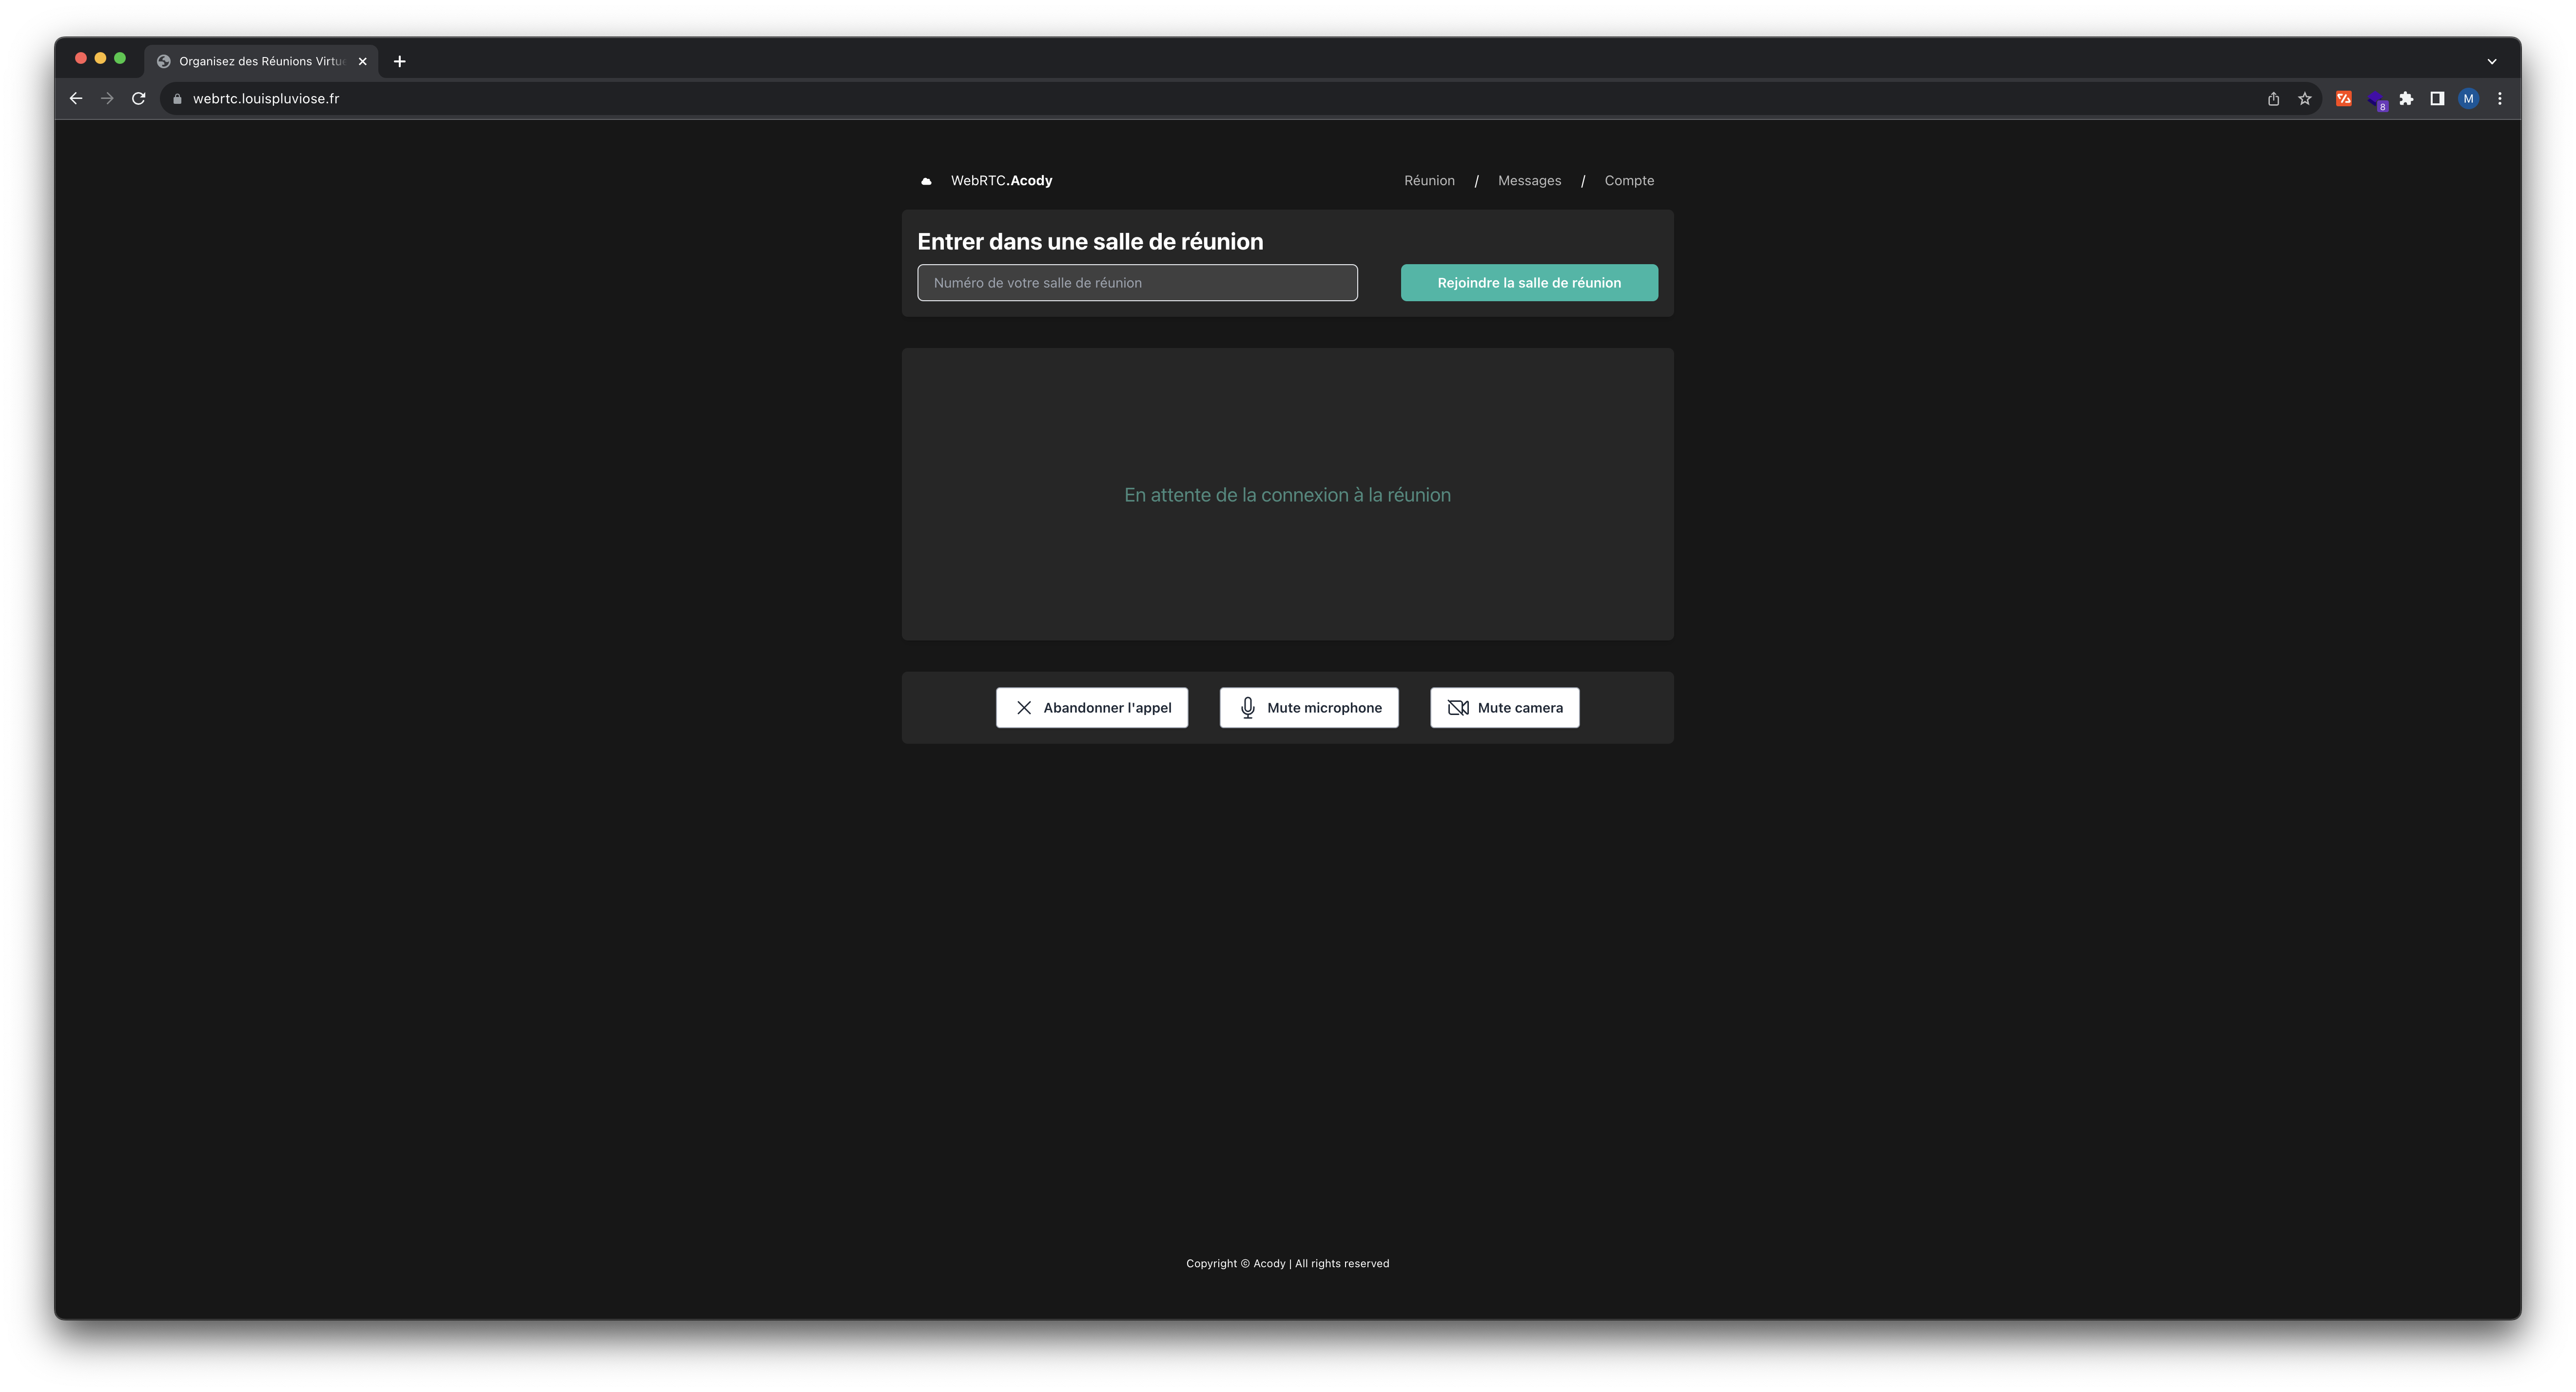
\includegraphics[width=0.6\textwidth]{images/PageReunionApplication.png}
    \caption{Page Réunion de l'application}
\end{figure}

\begin{figure}[h]
    \centering
    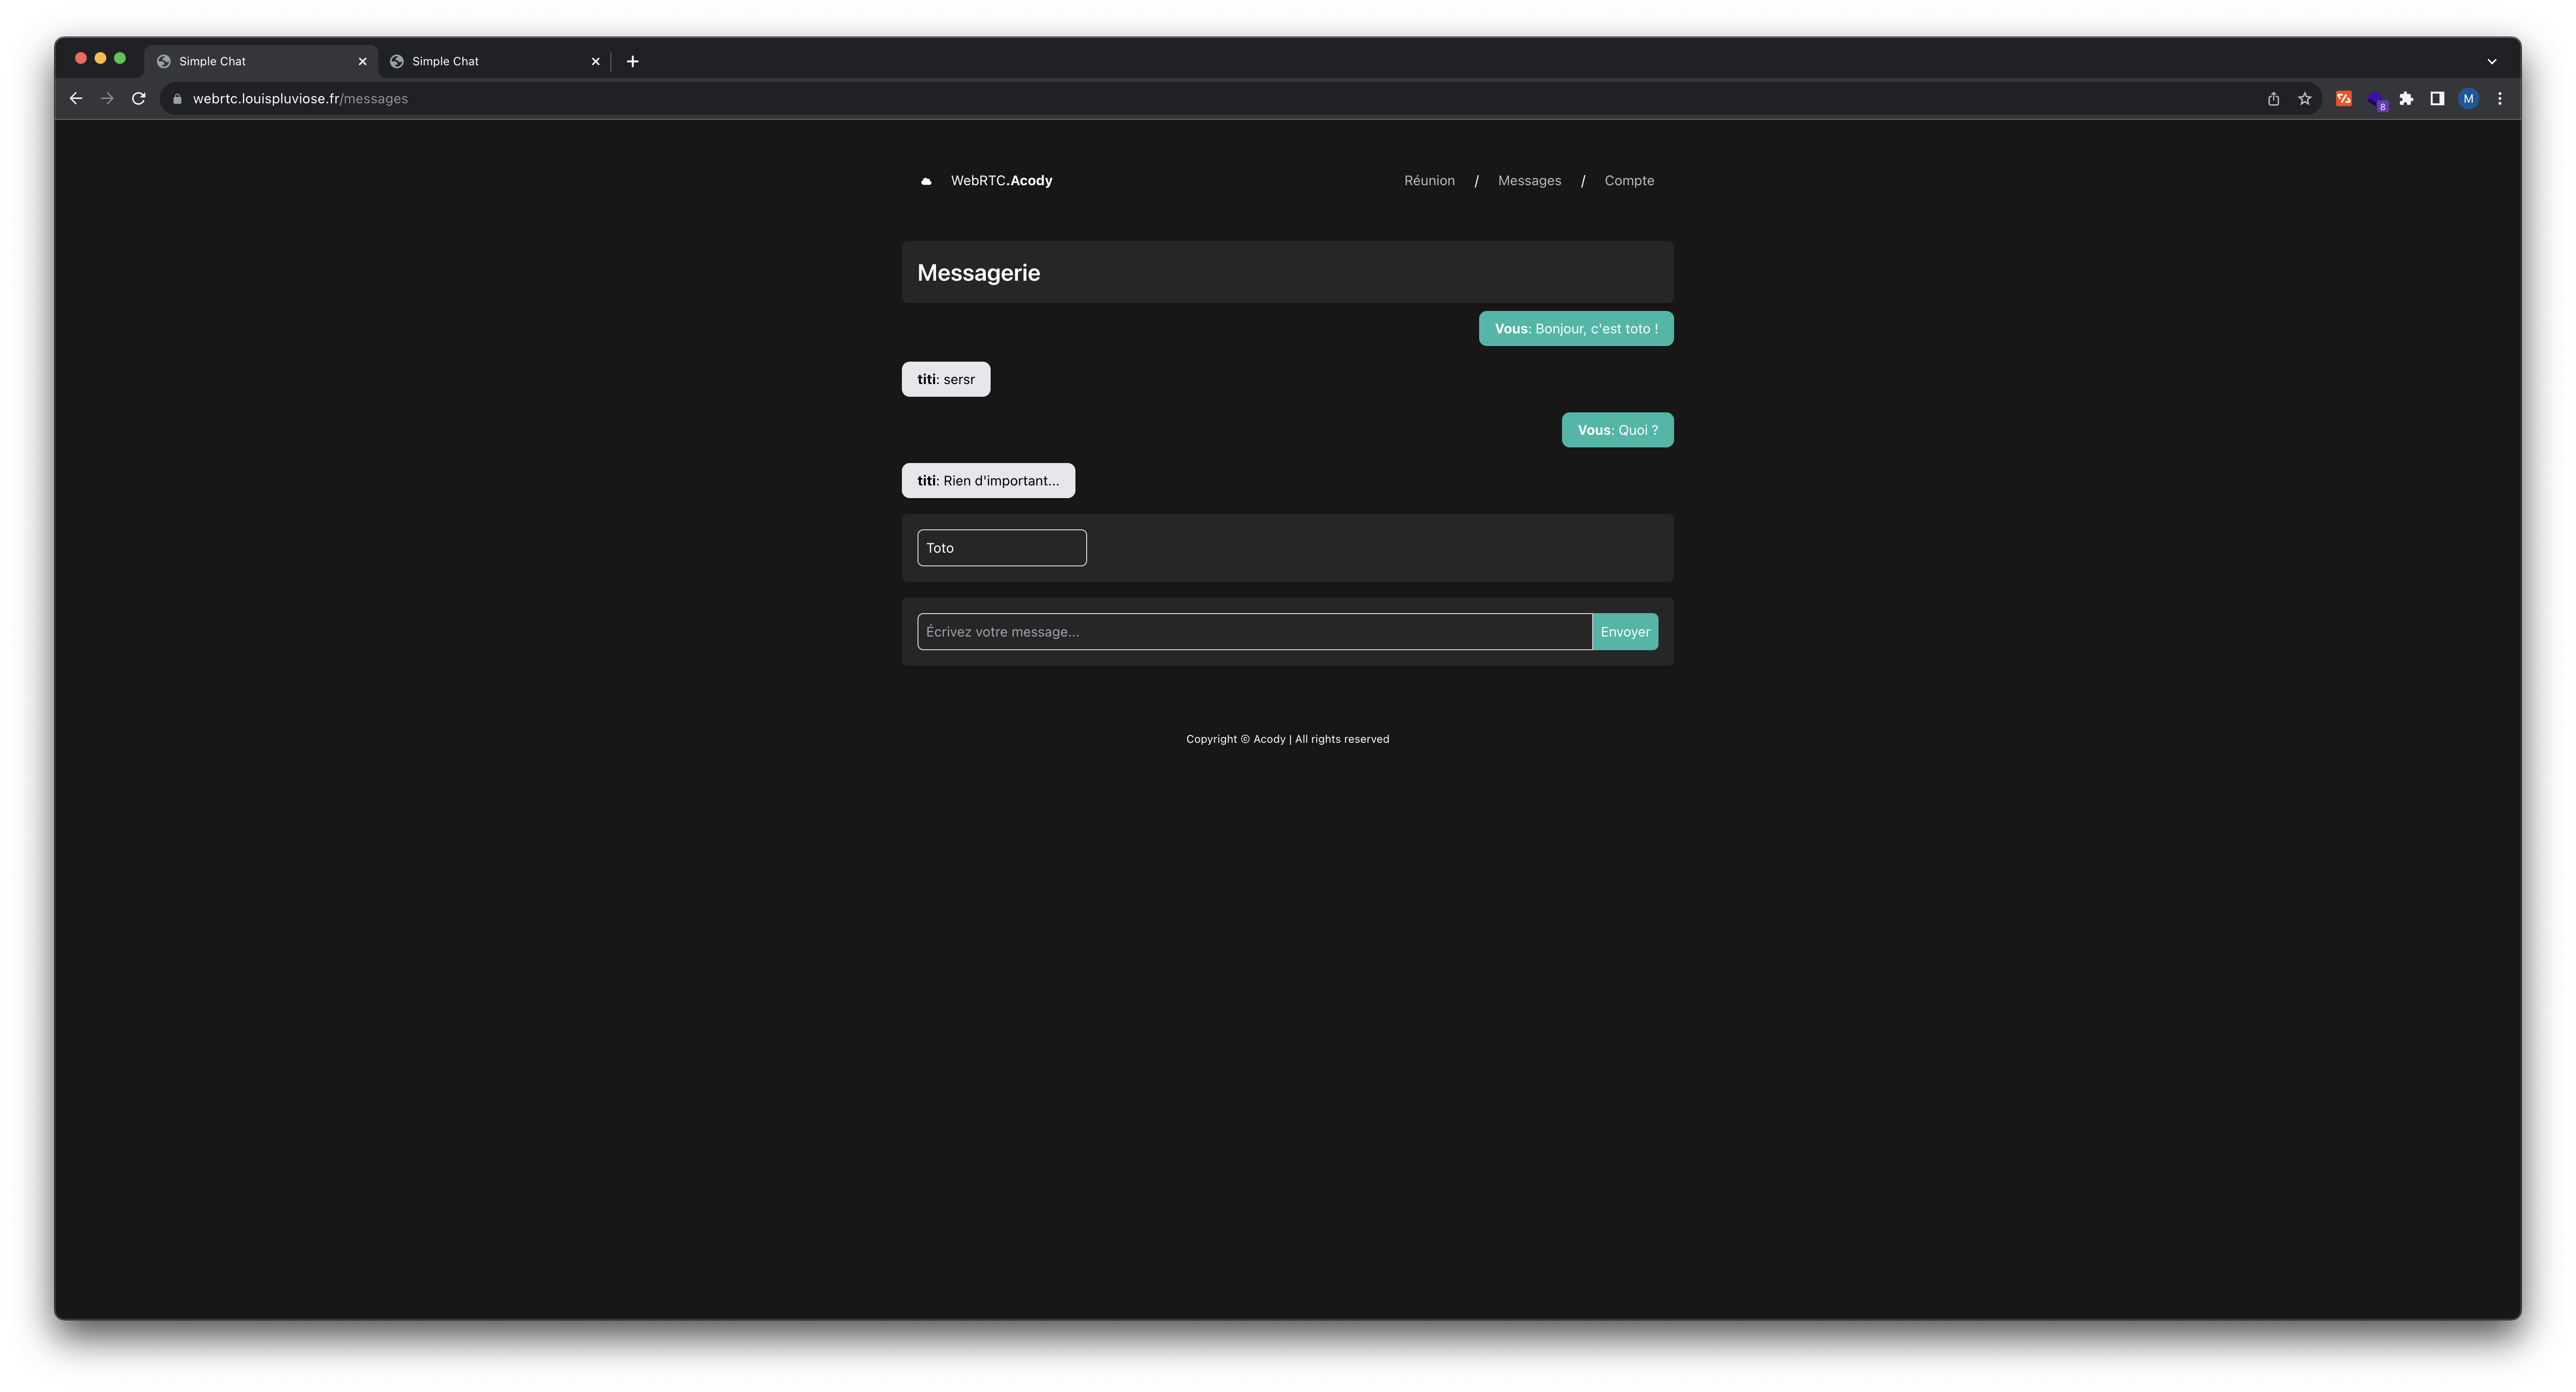
\includegraphics[width=0.6\textwidth]{images/PageMessagerieApplication.png}
    \caption{Page Messagerie de l'application}
\end{figure}

\subsection{Technologies utilisées}
\subsubsection{Astro.js - Framework frontend utilisé}
Nous avons utilisé le framework Astro.js pour la réalisation de la partie frontend de notre application web. 
C'est un framework récent sur le marché qui adopte une approche "server-first", privilégiant le rendu côté serveur par rapport au rendu côté client dans le navigateur. 
Cela offre des performances très élevées, ce qui nous intéresse dans le cas de notre projet.
Également dans ce framework, tout est réuni dans un seul fichier texttt{.astro} : HTML, CSS et JavaScript. 
De plus, sa compatibilité avec des frameworks tels que "TailwindCSS" et "React.js" nous a permis d'appliquer un design moderne et convivial pour l'utilisateur.


\subsubsection{TailwindCSS et React.js}
Tailwind CSS est un framework CSS utilitaire qui simplifie le développement et la stylisation des interfaces utilisateur. Contrairement aux frameworks CSS traditionnels basés sur des composants prédéfinis, Tailwind CSS fournit des classes utilitaires directement applicables dans le code HTML. Ces classes permettent de définir rapidement et de manière cohérente des styles tels que la couleur, la taille, la marge, le rembourrage, etc. L'approche de Tailwind CSS encourage une flexibilité accrue tout en offrant une base solide pour la conception.

React.js est une bibliothèque JavaScript développée par Facebook pour la construction d'interfaces utilisateur interactives. React utilise une approche basée sur les composants, permettant de créer des morceaux d'interface réutilisables et modulaires. Cette approche facilite la gestion de l'état de l'application et la mise à jour dynamique de l'interface en réponse aux changements.

Dans le cadre de notre projet, nous avons utilisé Tailwind CSS pour simplifier la stylisation en exploitant ses classes utilitaires directement dans le code HTML. Cela a accéléré le processus de conception en nous permettant de définir rapidement et de manière cohérente les styles des éléments.

Parallèlement, nous avons intégré React.js pour structurer l'interface utilisateur de manière modulaire. Les composants React ont été utilisés pour diviser l'application en parties réutilisables, facilitant ainsi la maintenance et la gestion de l'état global de l'application.

\subsection{Contexte de l'Application}
L'application vise à faciliter les réunions virtuelles en temps réel. Elle offre une plateforme pour la communication vidéo instantanée, améliorant ainsi la collaboration à distance. Les fonctionnalités clés comprennent la possibilité d'entrer dans une salle de réunion en utilisant un numéro spécifique, la gestion du son et de la caméra, ainsi que la capacité à abandonner les appels en un clic.
En plus des fonctionnalités de réunion vidéo en temps réel, l'application intègre également une fonctionnalité de messagerie pour une communication asynchrone entre les utilisateurs. Cette fonctionnalité permet aux utilisateurs d'échanger des messages textuels, complétant ainsi l'expérience de communication collaborative.

\subsubsection{Public Cible}
L'application cible un large éventail d'utilisateurs professionnels cherchant à optimiser leurs réunions virtuelles. Elle s'adresse particulièrement aux équipes travaillant à distance, aux entreprises cherchant à améliorer la communication interne et externe, ainsi qu'aux individus ayant besoin d'une solution efficace pour les réunions en ligne.

\subsubsection{Objectifs de l'Application (Réunions)}
\begin{enumerate}
    \item \textbf{Faciliter les Réunions Virtuelles :} Offrir une plateforme conviviale pour l'organisation de réunions virtuelles.
    \item \textbf{Communication Vidéo en Temps Réel :} Permettre des appels vidéo en temps réel pour une interaction plus dynamique.
    \item \textbf{Simplicité d'Utilisation :} Assurer une expérience utilisateur intuitive pour maximiser l'adoption de l'application.
    \item \textbf{Optimiser la Collaboration à Distance :} Fournir des fonctionnalités simples et efficaces pour améliorer la collaboration à distance.
\end{enumerate}

\subsubsection{Objectifs de l'Application (Messagerie)}
\begin{enumerate}
    \item \textbf{Communication Asynchrone :} Fournir une plateforme de messagerie pour permettre des échanges asynchrones entre les utilisateurs.
    \item \textbf{Facilité d'Utilisation :} Assurer une interface conviviale pour la saisie et l'envoi de messages.
    \item \textbf{Identité de l'Utilisateur :} Permettre aux utilisateurs de spécifier leur nom d'utilisateur pour une identification personnalisée.
\end{enumerate}

\subsubsection{Principales Fonctionnalités (Réunions)}
\begin{enumerate}
    \item \textbf{Entrée dans une Salle de Réunion :} Les utilisateurs peuvent rejoindre une salle de réunion en saisissant un numéro spécifique.
    \item \textbf{Gestion du Son et de la Caméra :} Contrôle de la fonction audio et vidéo pour une expérience personnalisée.
    \item \textbf{Abandonner les Appels en un Clic :} Facilité pour quitter rapidement une réunion.
    \item \textbf{Affichage Vidéo en Temps Réel :} Possibilité de visualiser les flux vidéo en temps réel des participants.
\end{enumerate}

\subsubsection{Principales Fonctionnalités (Messagerie)}
\begin{enumerate}
    \item \textbf{Saisie de Nom d'Utilisateur :} Les utilisateurs peuvent entrer leur nom d'utilisateur pour une identification personnalisée.
    \item \textbf{Saisie de Message :} Interface pour la saisie et l'envoi de messages texte.
    \item \textbf{Affichage des Messages :} Les messages échangés sont affichés dans une interface dédiée.
    \item \textbf{Styles Différenciés :} Les messages de l'utilisateur actuel sont stylisés différemment pour une distinction visuelle.
\end{enumerate}

\subsubsection{Implémentation Technique (Réunions)}
\begin{enumerate}
    \item \textbf{Utilisation de Socket.io :} Les connexions peer-to-peer WebRTC sont établies via les événements de socket, notamment les événements \texttt{room\_created}, \texttt{room\_joined}, et \texttt{start\_call}.
    \item \textbf{RTCPeerConnection :} Pour créer et gérer les connexions peer-to-peer.
    \item \textbf{Interface Utilisateur :} La partie vidéo est divisée en un conteneur local et plusieurs conteneurs distants.
\end{enumerate}

\subsubsection{Implémentation Technique (Messagerie)}
\begin{enumerate}
    \item \textbf{Utilisation de Socket.io :} La messagerie utilise Socket.io pour la gestion des communications en temps réel.
    \item \textbf{Identifiant Unique de l'Utilisateur :} Chaque utilisateur est associé à un identifiant unique généré au moment de la connexion.
    \item \textbf{Événements Socket.io :} L'application utilise des événements Socket.io tels que 'connect' et 'chat\_message' pour gérer la communication.
\end{enumerate}

\newpage
\section{Analyse UI/UX}

\subsection{Disposition principal de l'application}

Un composant principal de l'application est mise en place pour gérer la disposition globale de l'application. Ce composant est utilisé pour encapsuler les composants de navigation et de pied de page, ainsi que le contenu de la page. Il est également utilisé pour définir les paramètres globaux de l'application, tels que la couleur de fond,la taille maximale de la page, la police et etc... \newline
Le code source est présent en annexe (voir Annexe 4). Voici une explication technique à travers différents points sur la structure du composant principal de l'application.

\subsubsection{Structure Globale}
Le code présente une structure HTML en Astro, avec l'inclusion de composants tels que \texttt{MainHead}, \texttt{Nav}, et \texttt{Footer}. Le corps de la page est défini avec des classes CSS pour la mise en page, la couleur de fond et la taille maximale.

\subsubsection{Barre de Navigation (\texttt{<Nav />})}
La barre de navigation est intégrée via le composant \texttt{Nav}. Cependant, le code spécifique à la barre de navigation elle-même n'est pas inclus ici. 
Nous importons le composant \texttt{Nav} depuis le fichier \texttt{Nav.astro} (voir Annexe 3).

\subsubsection{Styles Globaux}
Des styles globaux sont définis, notamment pour le corps de la page, la police (San Francisco) et la couleur de fond. 
\subsubsection{Police San Francisco}
Une police personnalisée, San Francisco, est intégrée via \texttt{@font-face}. Cela peut contribuer à l'esthétique globale de la page, mais la police étant chargée depuis un lien externe, la vitesse de chargement peut être affectée.

\subsubsection{Utilisation de Variables Dynamiques}
Des variables telles que \texttt{title}, \texttt{seoTitle}, et \texttt{seoDesc} provenant du composant \texttt{MainHead} sont présentes. Cela permet une personnalisation dynamique du titre et de la description SEO.

\newpage
\subsection{Navigation}
La dispostiion et la navigation au sein de l'application s'effectue via une barre de navigation positionnée en haut de la page. Cette barre comprend deux boutons : "Réunions" et "Messages". L'utilisateur final est ainsi invité à faire son choix à travers cette barre de navigation, lui offrant une manière claire et accessible d'accéder aux fonctionnalités désirées.

\begin{figure}[h]
    \centering
    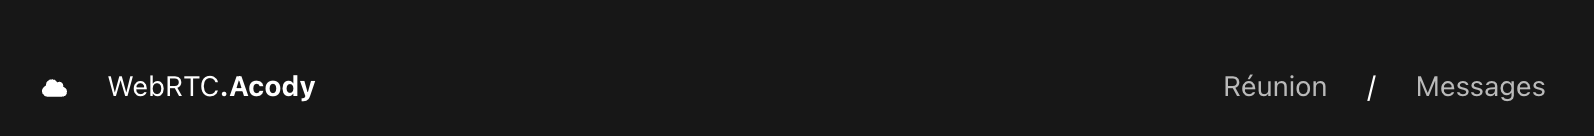
\includegraphics[width=0.6\textwidth]{images/NavBarPC.png}
    \caption{Barre de navigation sur un écran large}
\end{figure}

\subsubsection{Réalisation Technique}
Le code source est présent en annexe (voir Annexe 3 - 15.1.3). Voici une explication technique à travers différents points sur la structure de la "NavBar" (barre de navigation) de l'application.

\begin{enumerate}
    \item \textbf{Structure HTML et classes CSS :}
    - La structure de la barre de navigation est définie dans une balise \texttt{header}.
    - La classe \texttt{lg:flex} rend la barre de navigation flexible sur les écrans de taille large.
    - La balise \texttt{Astronav} encapsule l'ensemble de la barre de navigation.

    \item \textbf{Logo et titre :}
    - Un logo représenté par un fichier SVG est inclus, utilisant la classe \texttt{icon}.
    - Le titre de la page, "WebRTC.Acody," est placé à côté du logo et est stylisé avec des classes CSS.

    \item \textbf{Bouton de menu pour les écrans de taille réduite :}
    - Pour les écrans de taille réduite (inférieure à lg), un bouton de menu est affiché grâce à la classe \texttt{icon-menus}.

\end{enumerate}

\begin{figure}[h]
    \centering
    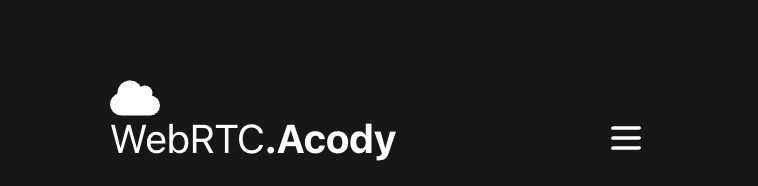
\includegraphics[width=0.6\textwidth]{images/NavBarMobileClose.png}
    \caption{Bouton de menu pour les écrans de taille réduite}
\end{figure}

\begin{enumerate}
    \item[4.] \textbf{MenuItems et liens de navigation :}
    - La balise \texttt{MenuItems} enveloppe la liste de navigation et la classe \texttt{hidden} la rend initialement invisible sur les écrans larges.
    - La liste de navigation est structurée avec des liens vers les sections du site telles que "Réunion," "Messages".

\end{enumerate}

\begin{figure}[h]
    \centering
    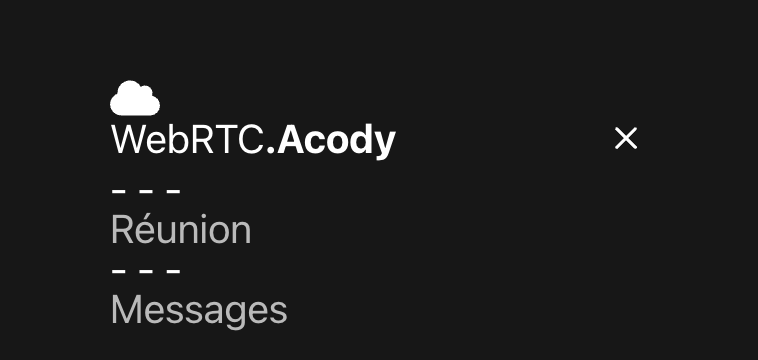
\includegraphics[width=0.6\textwidth]{images/NavBarMobileOpen.png}
    \caption{Menu ouvert sur les écrans de taille réduite}
\end{figure}

\begin{enumerate}
    \item[5.] \textbf{Styles CSS :}
    - Des styles CSS personnalisés sont définis pour les séparateurs, les liens de la liste, le survol des liens, l'opacité, et les filtres d'image.
    - Des classes telles que \texttt{separator-mob} sont utilisées pour ajuster le style en fonction de la taille de l'écran.
    - Les filtres d'image, tels que \texttt{hue-rotate}, sont appliqués pour des effets visuels lors du survol.

    \item[6.] \textbf{Media Queries :}
    - Des règles de media queries sont utilisées pour adapter le style en fonction de la largeur de l'écran.
    - Les séparateurs sont masqués sur les écrans de taille réduite, et des styles spécifiques sont appliqués aux éléments pour une meilleure lisibilité.
\end{enumerate}

\subsubsection{Expérience utilisateur}
\begin{enumerate}
    \item[1.] \textbf{Clarté et Simplicité :}
    - La barre de navigation est simple et claire, avec seulement deux boutons principaux : "Réunions" et "Messages". Cela évite toute confusion et facilite la navigation.

    \item[2.] \textbf{Logo et Titre :}
    - L'inclusion d'un logo et du titre "WebRTC.Acody" renforce l'identité visuelle de la page. Cela améliore la reconnaissance du projet et aide les utilisateurs à comprendre le contexte de la page.
  
    \item[3.] \textbf{Adaptabilité pour les Petits Écrans :}
    - La barre de navigation est conçue pour s'adapter aux petits écrans. L'utilisation d'un bouton de menu (MenuIcon) pour les écrans de taille réduite montre une considération pour les utilisateurs sur des appareils mobiles.

    \item[4.] \textbf{Effets Visuels au Survole :}
    - Les effets visuels au survol, tels que le changement d'opacité et la rotation de teinte, ajoutent une dimension interactive à la barre de navigation, améliorant l'expérience visuelle.

\end{enumerate}
\newpage
\subsection{Page - Réunion}

La page de réunion Webrtc représente le cœur de l'application WebRTC. Conçue pour faciliter les réunions virtuelles en temps réel, cette page offre une interface conviviale et des fonctionnalités robustes de communication vidéo. L'objectif est de permettre aux utilisateurs de se connecter facilement, de participer à des réunions de manière efficace, tout en offrant une expérience visuelle optimale. 

\begin{figure}[h]
  \centering
  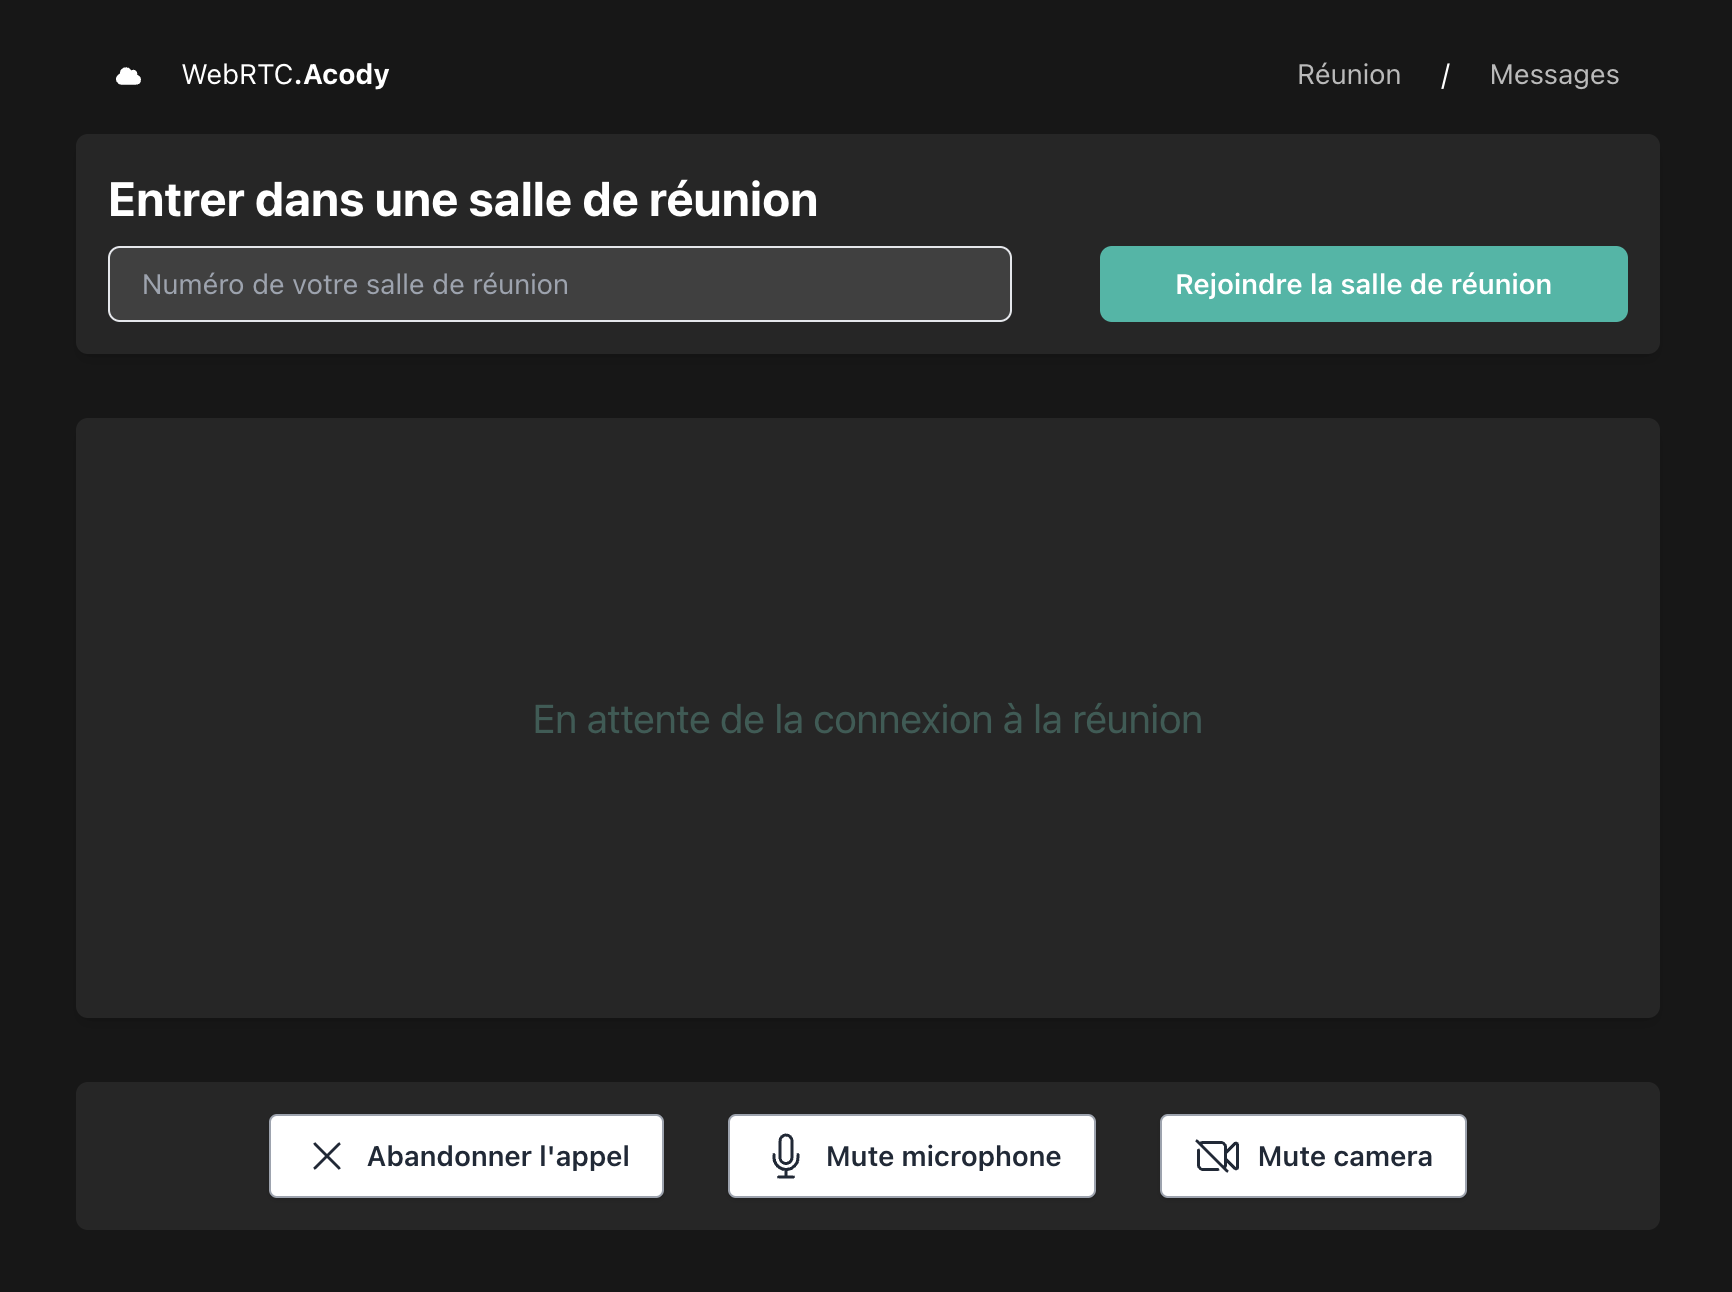
\includegraphics[width=0.6\textwidth]{images/ReunionPres.png}
  \caption{La page de réunion}
\end{figure}

\subsubsection{Réalisation Technique}
La page de réunion Webrtc est élaborée avec une approche technique solide, combinant l'utilisation d'un composant de mise en page et des styles CSS soigneusement définis

\begin{enumerate}
    \item \textbf{Composant de Mise en Page :} L'utilisation du composant \texttt{Layout} assure une gestion centralisée du contenu, améliorant ainsi la maintenance.
    \item \textbf{Styles CSS pour Vidéos :} Les règles CSS détaillées assurent une disposition précise des vidéos, garantissant une expérience visuelle optimale.
    \item \textbf{Affichage Conditionnel Dynamique :} Des règles conditionnelles sont utilisées pour ajuster dynamiquement l'affichage en fonction de l'état de la page.
\end{enumerate}

\subsubsection{Expérience Utilisateur}
La page de réunion Webrtc offre une expérience utilisateur immersive et interactive, grâce à des fonctionnalités pensées pour faciliter les interactions en temps réel.

\begin{enumerate}
    \item \textbf{Interface Conviviale :} La mise en page soigneusement conçue assure une navigation intuitive et une utilisation facile.
    \item \textbf{Visualisation Vidéo Optimal :} Les dimensions et les positions des vidéos sont gérées de manière à offrir une présentation visuelle optimale.
    \item \textbf{Interaction Intuitive :} Des boutons d'action avec des icônes permettent des actions rapides, améliorant ainsi l'expérience utilisateur.
    \item \textbf{Affichage Conditionnel :} Certains éléments sont dynamiquement affichés ou masqués en fonction de l'état de la page, optimisant ainsi l'interface utilisateur.
\end{enumerate}


\newpage
\subsection{Page - Messagerie}

Conçue pour simplifier les échanges professionnels, cette page présente une interface utilisateur conviviale et des fonctionnalités de messagerie robustes.

\begin{figure}[h]
  \centering
  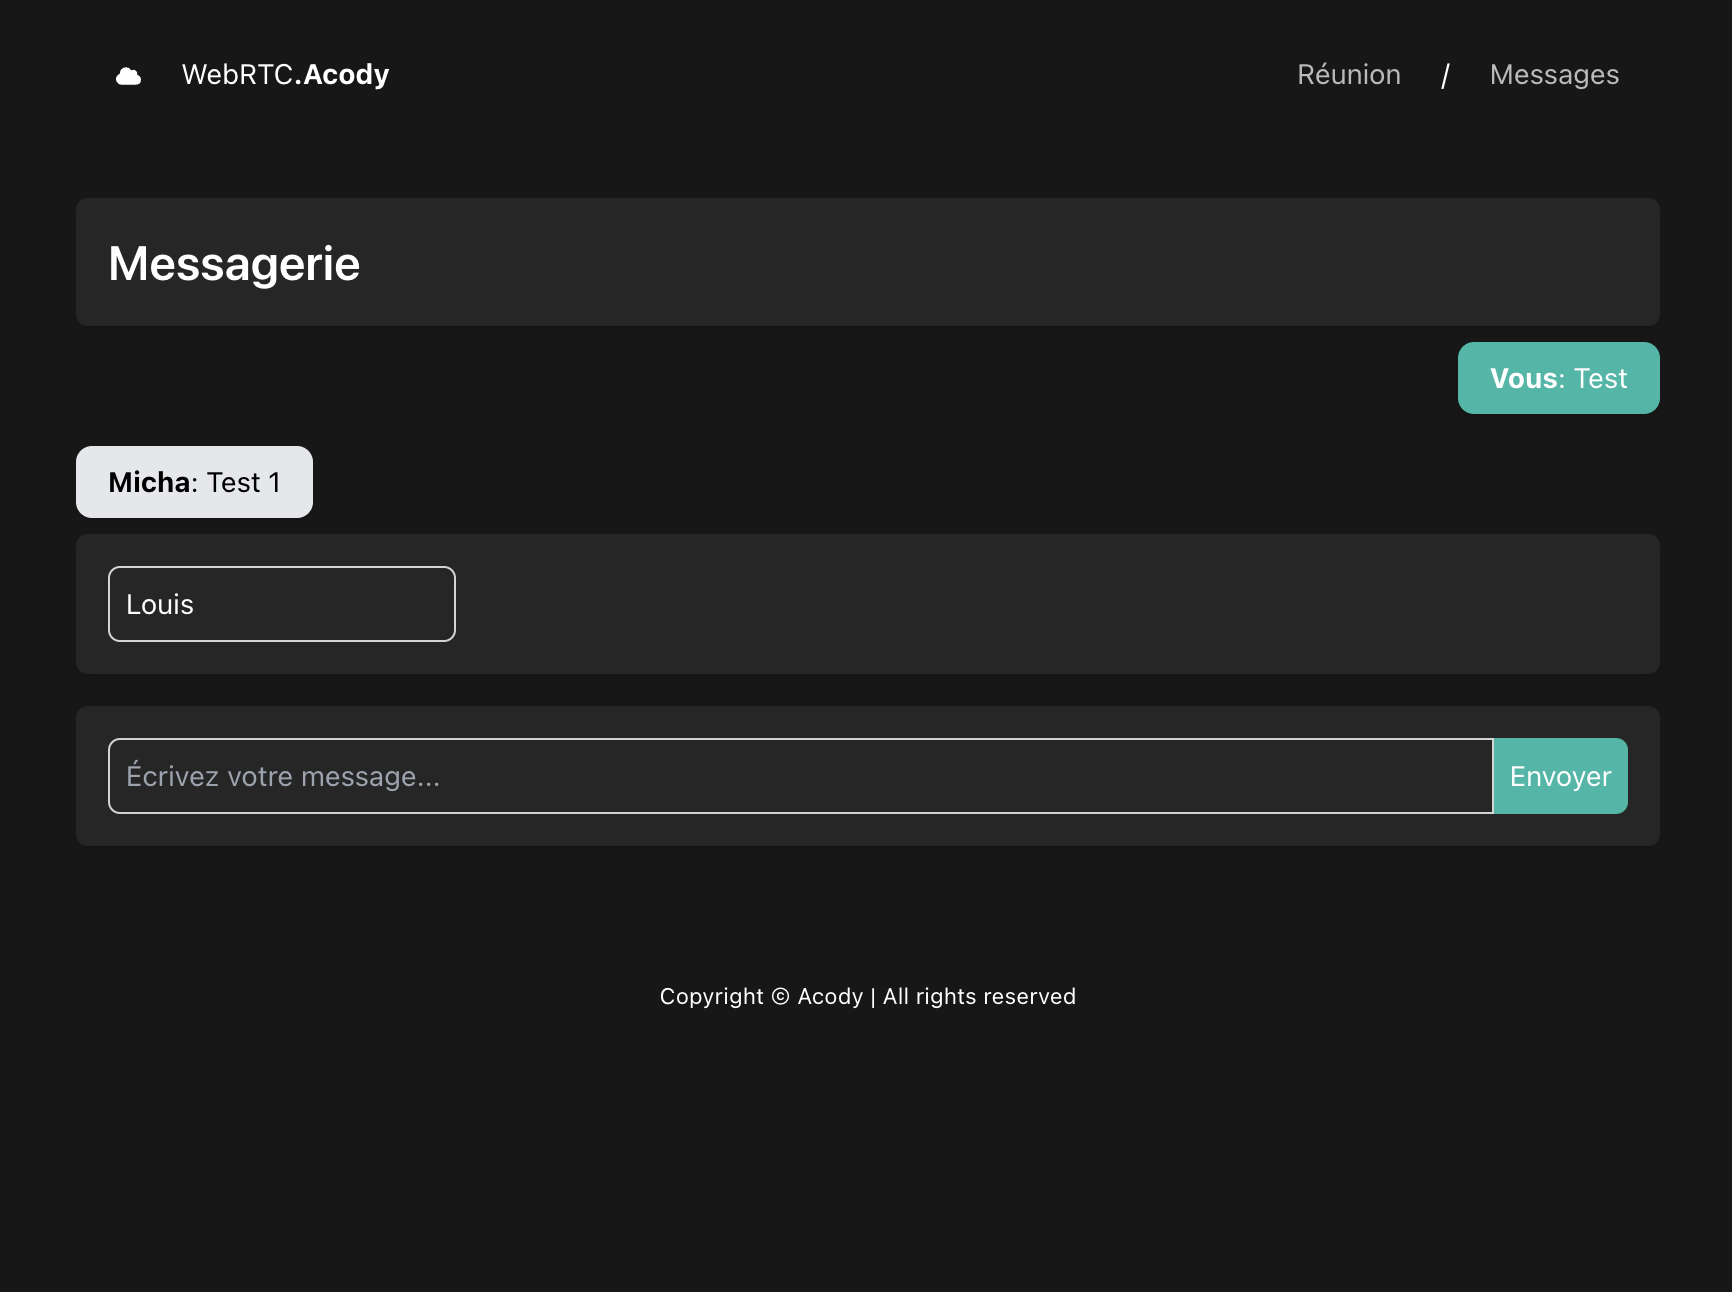
\includegraphics[width=0.6\textwidth]{images/MessageriePres.png}
  \caption{La page de Messagerie}
\end{figure}

\subsubsection{Réalisation Technique}
La page de messagerie Webrtc est construite avec une approche technique solide, tirant parti du composant de mise en page et de styles CSS détaillés.

\begin{enumerate}
    \item \textbf{Composant de Mise en Page :} L'utilisation du composant \texttt{Layout} permet une gestion centralisée du contenu, simplifiant ainsi la maintenance.
    \item \textbf{Styles CSS pour la Messagerie :} Des règles CSS détaillées sont employées pour styliser la zone de chat, assurant une expérience visuelle cohérente.
\end{enumerate}

\subsubsection{Expérience Utilisateur}
La page de messagerie Webrtc offre une expérience utilisateur immersive grâce à des fonctionnalités dédiées à la communication en temps réel.

\begin{enumerate}
    \item \textbf{Interface Intuitive :} La section de messagerie est conçue avec une mise en page claire, facilitant la lecture et l'envoi de messages.
    \item \textbf{Chat en Temps Réel :} Les messages s'affichent dynamiquement, offrant une communication instantanée et fluide.
    \item \textbf{Gestion Simple des Utilisateurs :} L'ajout d'un nom d'utilisateur est facilité par une zone de saisie dédiée, permettant une personnalisation rapide.
    \item \textbf{Envoi Facile de Messages :} La zone de saisie de message et le bouton "Envoyer" simplifient le processus d'envoi de messages.
\end{enumerate}

\newpage
\subsection{Pied de page - Footer}
Le pied de page (footer) de l'application est défini de manière concise et centrée, 
avec une structure HTML minimale. Voici une explication rapide du code du pied de page.

\begin{figure}[h]
  \centering
  
\includegraphics[width=0.6\textwidth]{images/PiedDePage.png}
  \caption{Le pied de page}
\end{figure}

\subsubsection{Réalisation Technique}
\begin{enumerate}
  \item[1.] \textbf{Structure HTML :}
  \newline- La balise \texttt{<footer>} encadre le contenu du pied de page.\newline
  - Les classes CSS comme \texttt{`mt-auto`, `py-4`, et `text-center`} sont utilisées pour ajuster la présentation, offrant une marge supérieure automatique, un espacement vertical optimal, et un centrage du texte sur tous les écrans.


  \item[2.] \textbf{Dynamisme de l'Année :}
  \newline
  - La balise \texttt{<span id="copyright"></span>} permet la mise à jour dynamique de l'année actuelle. c'est effectué grace à un simple JavaScript.
\end{enumerate}

\subsubsection{Expérience Utilisateur}
Le pied de page assure une expérience utilisateur enrichissante en combinant une présentation soignée avec des effets visuels interactifs.

\begin{enumerate}
  \item[1.] \textbf{Styles Visuels des Liens :}
  \newline - Les liens dans le pied de page bénéficient d'une amélioration visuelle lors du survol.\newline
  - Une transition fluide d'opacité et une rotation de teinte apportent un dynamisme visuel agréable.
\end{enumerate}



\newpage
\section{Performances de l'application}

\subsection{Page Load Time}

Le rapport ci dessous, fourni par CloudFlare nous permet de voir les performances de notre application.\\

\verb|Temps de chargement global| : le temps de chargement de la page de 150 ms est exceptionnel et bien inférieur au temps de chargement moyen sur l'internet, qui dépasse souvent 1 000 ms. Cela indique que le backend et le réseau sont hautement optimisés.\\

\verb|Implications pour l'expérience utilisateur| : Un temps de chargement rapide, tel que celui obtenu, est susceptible de contribuer à une expérience utilisateur positive, en réduisant les taux de rebond et en améliorant potentiellement les taux de conversion.\\
\verb|Avantages du rendu côté serveur (SSR)| : Le SSR fourni par Astro.js permet au contenu d'être rendu sur le serveur et envoyé au client sous la forme d'une page statique.\\
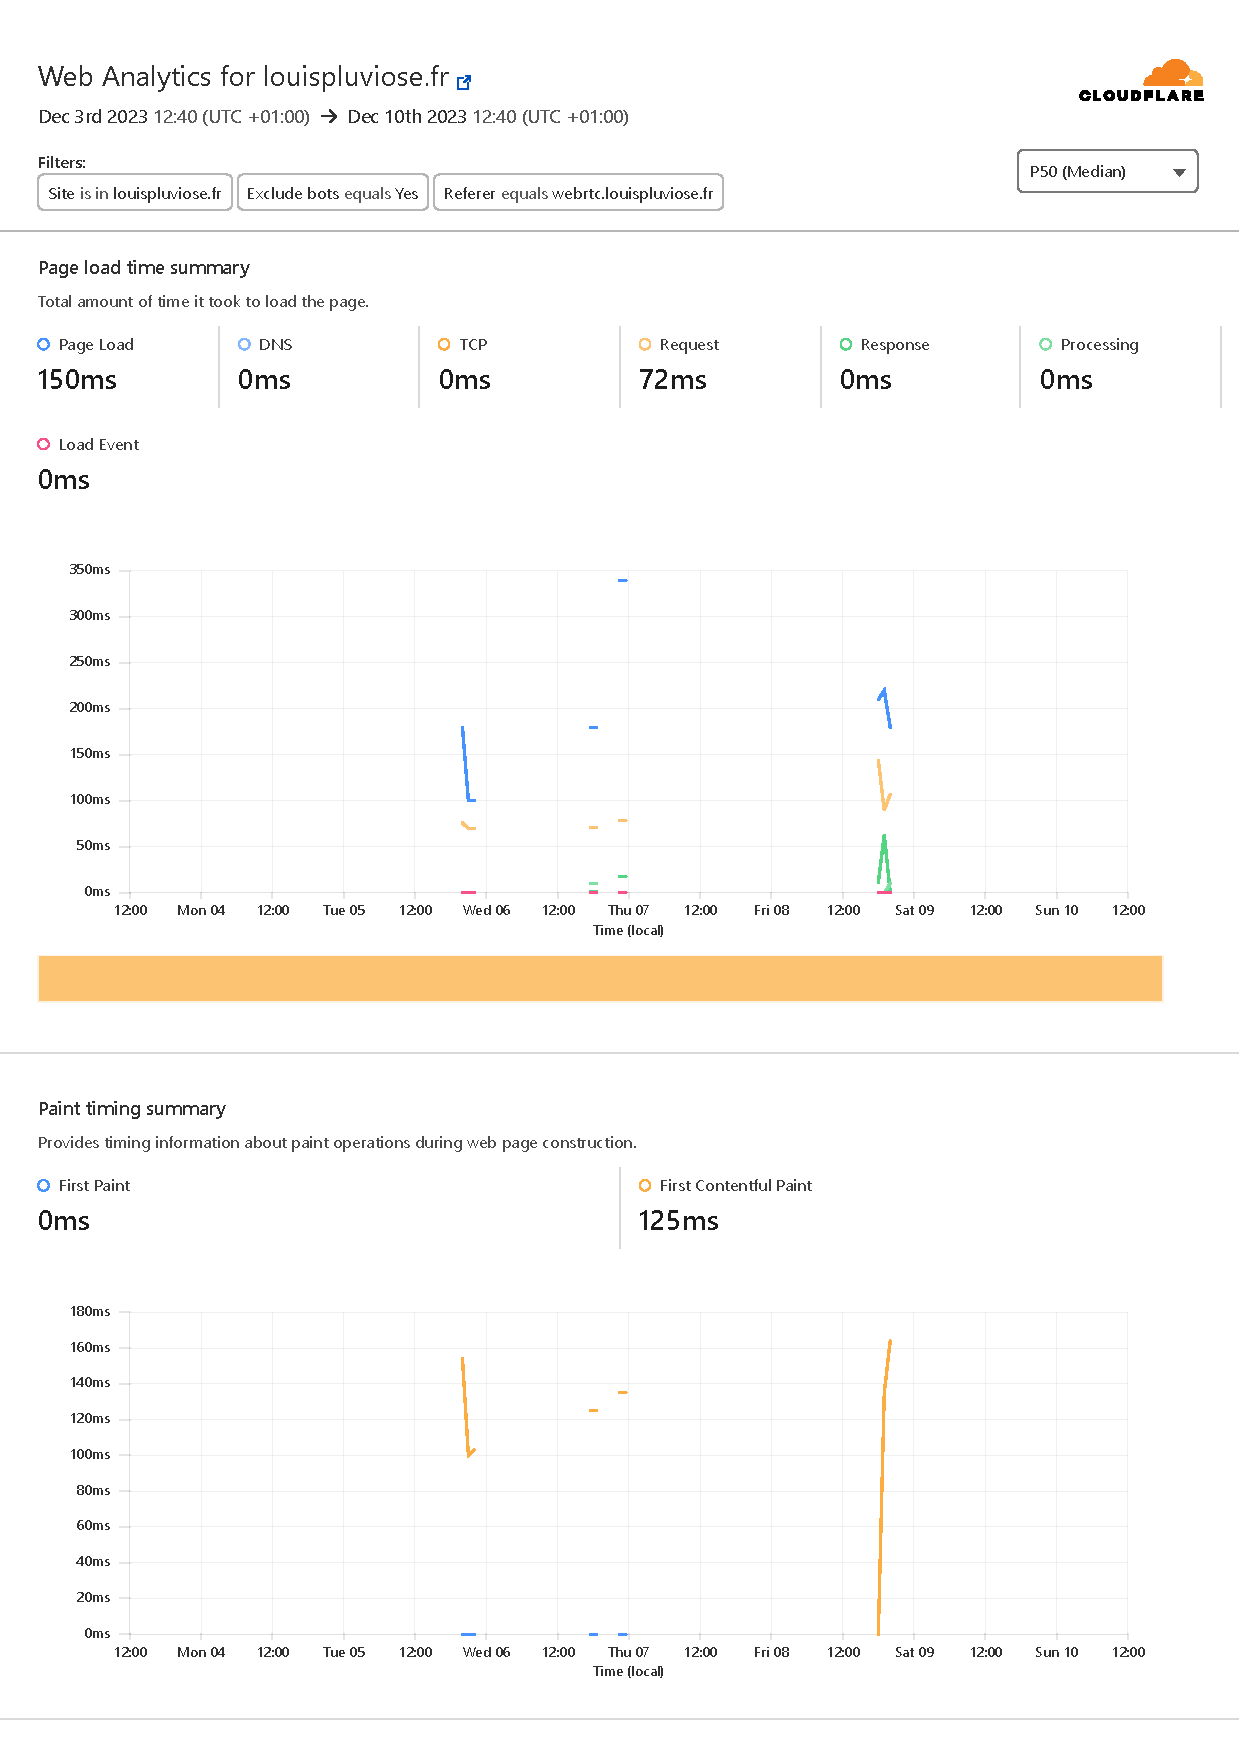
\includepdf[scale=0.75,pages=-]{pageloadtime.pdf}
\subsection{Core Web Vitals}

Le rapport ci dessous, fourni par CloudFlare nous permet de voir une analyse de l'expérience utilisateur de notre application.\\

Le rapport montre d'excellentes mesures de performance pour votre application. Le Largest Contentful Paint (LCP) pour différents percentiles (P50, P75, P90, P99) varie de 197 ms à 258 ms, ce qui est bien en deçà du seuil requis pour une bonne expérience utilisateur. Ces mesures indiquent que votre application charge toujours rapidement l'élément de contenu le plus volumineux pour la grande majorité des utilisateurs.\\

En outre, le délai de première entrée (FID) est bon à 100 \%, ce qui suggère que les utilisateurs peuvent interagir avec votre application presque immédiatement après le chargement du contenu. Cet aspect est crucial pour l'engagement et la fidélisation des utilisateurs.\\

Le décalage cumulatif de la mise en page (CLS) est bon à 92 \%, avec seulement 8 \% d'améliorations à apporter. Cela montre que la plupart des utilisateurs bénéficient d'une mise en page visuelle stable avec un minimum de décalages inattendus, ce qui est essentiel pour une bonne expérience utilisateur.\\

Dans l'ensemble, l'application de SSR avec Astro.js contribue clairement à une expérience utilisateur rapide et fiable à travers diverses mesures de performance.

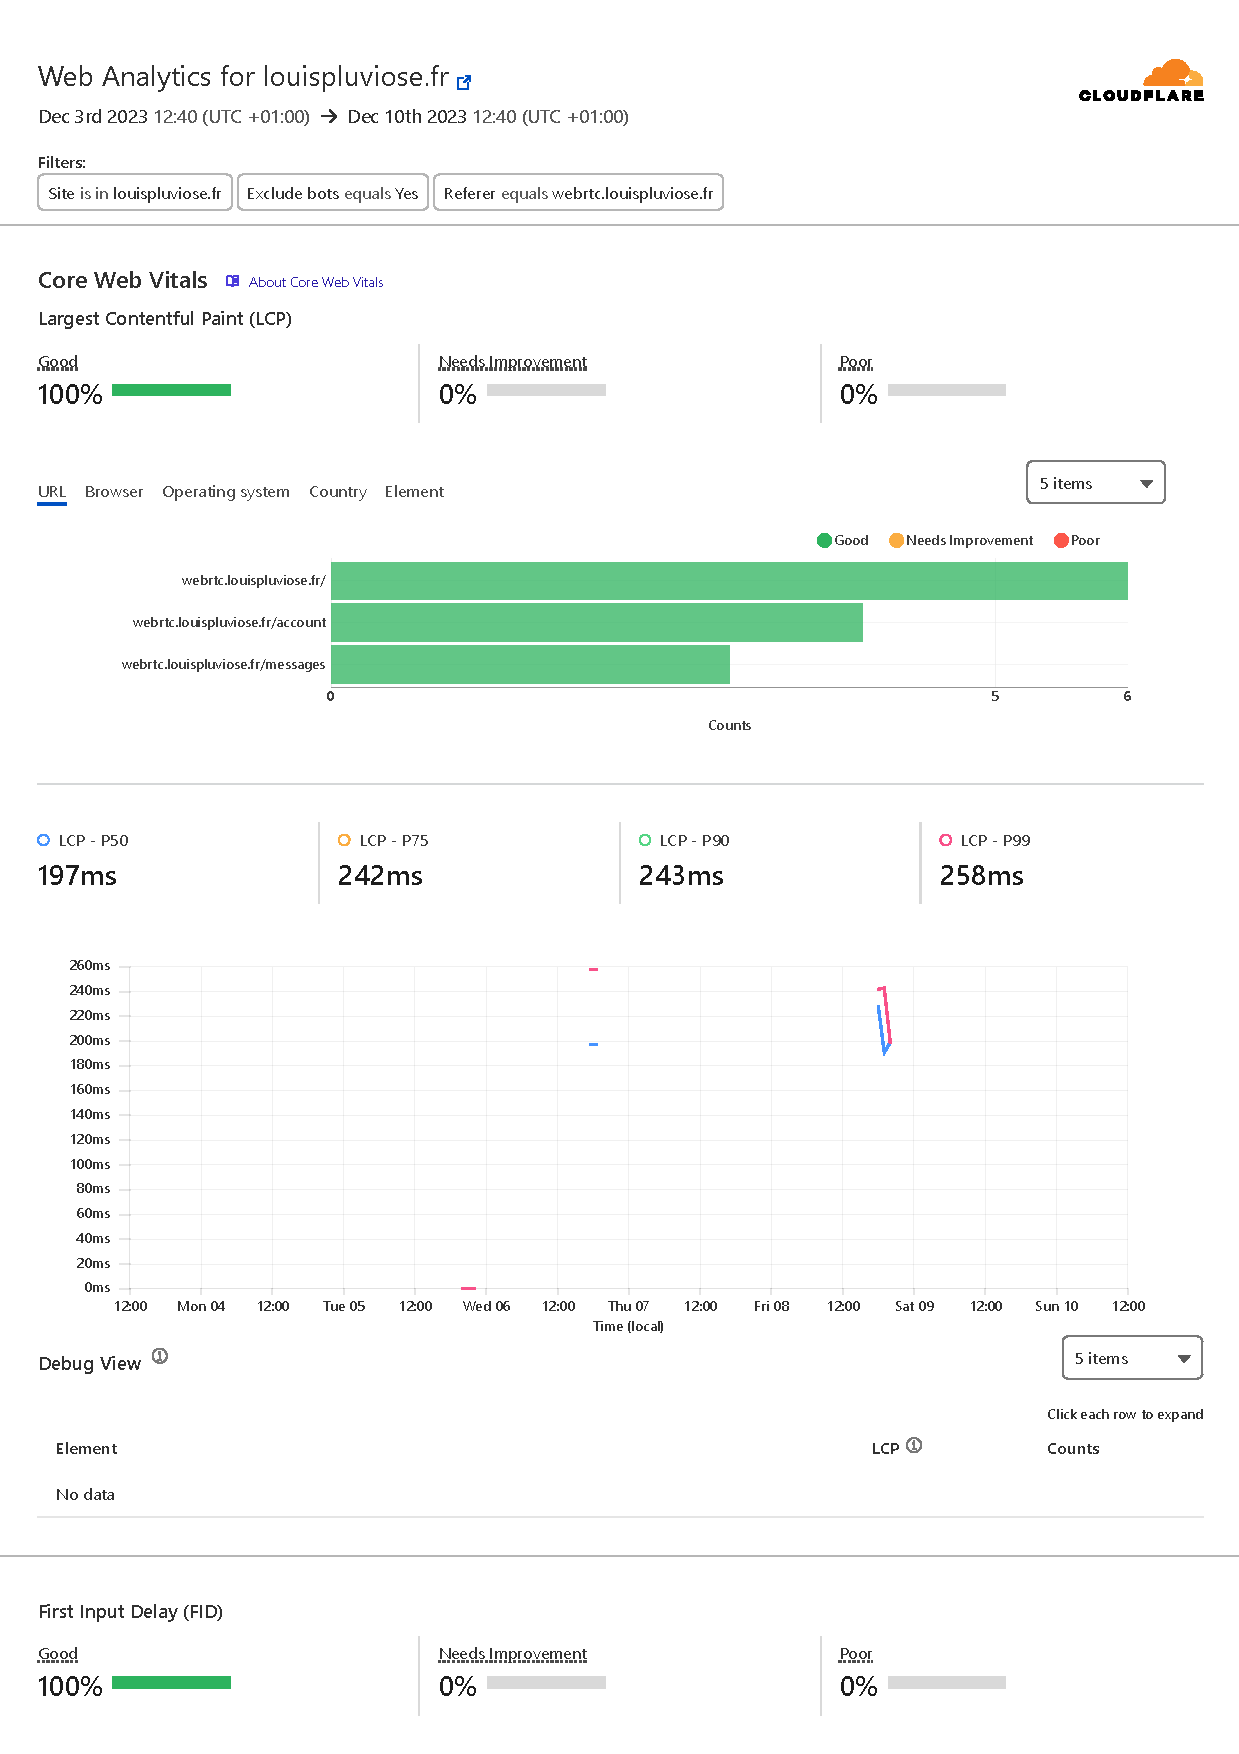
\includepdf[scale=0.75,pages=-]{corewebvitals.pdf}
\newpage
\section{Installation de l'application}

\subsection{Installation en dur}

ATTENTION : au préalable, il faut installer NodeJS et NPM sur la machine !\\

Pour installer l'application en dur, il suffit de cloner le dépôt git suivant : \url{https://github.com/mIKIII77/SAE5.ROM.03} avec la commande\\ 
\verb|git clone https://github.com/mIKIII77/SAE5.ROM.03.git|\\

Ensuite, il faut naviger dans le dossier \verb|SAE5.ROM.03/webssr| et lancer la commande \verb|npm install| pour installer les dépendances.\\
Enfin, il faut lancer la commande \verb|npm run build| puis \verb|node ./run-server.mjs| pour lancer l'application.\\

\newpage

\section{Bugs}

\subsection{Bugs connus}

Nous avons pu détecter 3 bugs dans notre application.\\

\subsubsection{Premier bug}

Lors de certains appels, il arrive que la connexion se fasse mal et que un des interlocuteurs ne voit pas l'autre. Voici plusieurs façon de résolver ce problème :\\

\begin{itemize}
  \item 1 : Il faut recliquer sur le bouton "Rejoindre la réunion"
  \item 2 : Si le problème persiste, Recharger la page
  \item 3 : Si le problème persiste toujours, il faut quitter la salle et en rejoindre une nouvelle
\end{itemize}

\subsubsection{Deuxième bug}

Au moment de raccrocher l'appel, il se peut la vidéo de l'autre interlocuteur reste affichée. Pour résoudre ce problème, il faut rafraichir la page.\\

\subsubsection{Troisième bug}

Lors de certains appels, il se peut que l'affichage se fasse mal et que les vidéos des interlocuteurs se chevauchent. Pour résoudre ce problème, il faut rafraichir la page.\\

\subsection{Bugs inconnus}

Si vous rencontrez d'autres bugs, merci de nous les signaler à l'adresse suivante : \href{mailto:contact@louispluviose.fr}{contact@louispluviose.fr}.\\

\newpage

\section{Annexes}

\subsection{Code du frontend}

\subsubsection{Page - Réunions}

\begin{lstlisting}[language=HTML, caption={Page - Réunions}, label=Page - Reunions]

  ---
  import Layout from '../layouts/Layout.astro';
  ---
  <Layout
    seoTitle="Reunion Webrtc - Application de Communication Video en Temps Reel | Acody"
    seoDesc="Facilitez vos reunions professionnelles avec notre application de projet Webrtc. Effectuez des appels video en temps reel, abandonnez les appels en un clic, et gerez facilement le son et la camera. Optimisez votre collaboration a distance avec des fonctionnalites simples et efficaces."
  >
  
  
  <div class="flex flex-col bg-neutral-900 rounded-md">
    <div class="flex-none bg-neutral-800 p-4 rounded-md shadow-md flex flex-col">
      <h1 class="text-2xl font-bold"> Entrer dans une salle de reunion </h1>
      <div class="grid grid-rows-1 mt-2">
        <input id="room-input" name="room" class="w-full px-4 py-2 border rounded-md focus:outline-none focus:border-teal-500 bg-neutral-700 col-span-6" placeholder="Numero de votre salle de reunion" />
        <button id="connect-button" type="submit" class="font-semibold w-full bg-teal-500 text-white px-4 py-2 rounded-md hover:bg-teal-700 focus:outline-none col-start-8">
        Rejoindre la salle de reunion
        </button>
      </div>
    </div>
    
    <style type="text/css">
      body, html {
        margin: 0;
        padding: 0;
        height: 100%;
        overflow: hidden;
      }
    
      #video-chat-container {
        display: grid;
        grid-template-columns: 1fr 1fr; /* Deux colonnes /
        grid-template-rows: 1fr 1fr; / Deux rangees */
        gap: 10px;
        width: 100vw;
        height: 30vh;
        padding: 10px;
      }
    
      video {
        width: 50%;
        height: 40%;
        object-fit: cover;
      }
    
      #local-video {
        grid-row: 2;
        grid-column: 1;
      }
    
      .remote-video-1 {
        grid-row: 1;
        grid-column: 1;
      }
    
      .remote-video-2 {
        grid-row: 1;
        grid-column: 2;
      }
    
      .remote-video-3 {
        grid-row: 2;
        grid-column: 2;
      }
  
      .room-selection-container {
        display: none;
      }
      </style>
  
  
    <!-- Partie fixe pour la video avec une hauteur personnalisee -->
    <div class="relative flex-grow">
      <div class="sticky top-0 bg-neutral-800 p-4 rounded-md shadow-md h-16 my-8 min-h-[300px] flex items-center justify-center">
        <div class="rounded-md p-4 max-w-sm w-full mx-auto">
          <div class="animate-pulse">
            <h1 id="waitingText" class="text-teal-300 opacity-50 text-xl text-center">En attente de la connexion a la reunion</h1>
          </div>
  
        </div>
        <div id="room-selection-container" class="display: hidden">
          <h1>WebRTC video conference</h1>
          <label>Enter the number of the room you want to connect</label>
          <input id="room-input" type="text" />
          <button id="connect-button">CONNECT</button>
          </div>
        
          <div id="video-chat-container" class="video-position" style="display: none">
            <div id="local-video-container">
              <video id="local-video" autoplay muted></video>
            </div>
          <div id="remote-videos-container">
            <video id="remote-video-1"></video>
            <video id="remote-video-2"></video>
            <video id="remote-video-3"></video>
          </div>
      </div>
    </div>
  
    <!-- Contenu principal -->
    <div class="bg-neutral-800 p-4 rounded-md flex flex-col md:flex-row justify-center items-center space-y-4 md:space-y-0 md:space-x-8" data-astro-cid-j7pv25f6="">
      <button class="bg-white hover:bg-gray-100 text-gray-800 font-semibold py-2 px-4 border border-gray-400 rounded shadow flex items-center" id="hangup-button" data-astro-cid-j7pv25f6="">
        <svg xmlns="http://www.w3.org/2000/svg" fill="none" viewBox="0 0 24 24" stroke-width="1.5" stroke="currentColor" class="w-6 h-6 mr-2" data-astro-cid-j7pv25f6="">
          <path stroke-linecap="round" stroke-linejoin="round" d="M6 18L18 6M6 6l12 12" data-astro-cid-j7pv25f6=""></path>
        </svg>
        Abandonner l'appel
      </button>
    
      <button class="bg-white hover:bg-gray-100 text-gray-800 font-semibold py-2 px-4 border border-gray-400 rounded shadow flex items-center" id="toggle-mic-button" data-astro-cid-j7pv25f6="">
        <svg xmlns="http://www.w3.org/2000/svg" fill="none" viewBox="0 0 24 24" stroke-width="1.5" stroke="currentColor" class="w-6 h-6 mr-2" data-astro-cid-j7pv25f6="">
          <path stroke-linecap="round" stroke-linejoin="round" d="M12 18.75a6 6 0 006-6v-1.5m-6 7.5a6 6 0 01-6-6v-1.5m6 7.5v3.75m-3.75 0h7.5M12 15.75a3 3 0 01-3-3V4.5a3 3 0 116 0v8.25a3 3 0 01-3 3z" data-astro-cid-j7pv25f6=""></path>
        </svg>
        Mute microphone
      </button>
    
      <button class="bg-white hover:bg-gray-100 text-gray-800 font-semibold py-2 px-4 border border-gray-400 rounded shadow flex items-center" id="toggle-camera-button" data-astro-cid-j7pv25f6="">
        <svg xmlns="http://www.w3.org/2000/svg" fill="none" viewBox="0 0 24 24" stroke-width="1.5" stroke="currentColor" class="w-6 h-6 mr-2" data-astro-cid-j7pv25f6="">
          <path stroke-linecap="round" stroke-linejoin="round" d="M15.75 10.5l4.72-4.72a.75.75 0 011.28.53v11.38a.75.75 0 01-1.28.53l-4.72-4.72M12 18.75H4.5a2.25 2.25 0 01-2.25-2.25V9m12.841 9.091L16.5 19.5m-1.409-1.409c.407-.407.659-.97.659-1.591v-9a2.25 2.25 0 00-2.25-2.25h-9c-.621 0-1.184.252-1.591.659m12.182 12.182L2.909 5.909M1.5 4.5l1.409 1.409" data-astro-cid-j7pv25f6=""></path>
        </svg>
        Mute camera
      </button>
    </div>
  
    </div>
  </div>

\end{lstlisting}

\newpage

\subsubsection{Page - Messagerie}

\begin{lstlisting}[language=HTML, caption={Page - Messagerie}, label=Page - Messagerie]
  ---
  import Layout from '../layouts/Layout.astro';
  ---
  <Layout seoTitle="Messagerie Webrtc - Application de Communication Video en Temps Reel" seoDesc="Facilitez vos reunions professionnelles avec notre application de projet Webrtc. 
  Effectuez des appels video en temps reel, abandonnez les appels en un clic, et gerez facilement le son et la camera. 
  Optimisez votre collaboration a distance avec des fonctionnalites simples et efficaces.">
    <div class="bg-neutral-800 text-white p-4 rounded-md shadow-md mt-8">
      <h1 class="text-2xl font-semibold">Messagerie</h1>
    </div>
  
    <!-- Zone de chat (ajoutee) -->
    <div id="messages" class="messages-container">
      <!-- Les messages s'afficheront ici -->
    </div>
  
  
    <!-- Zone de saisie de nom d'utilisateur -->
    <div class="bg-neutral-800 p-4 rounded-md shadow-md mb-4 mt-4">
      <input
        id="username"
        type="text"
        placeholder="Entrez votre nom d'utilisateur..."
        class="flex-1 p-2 border border-neutral-300 rounded-md bg-neutral-800"
      />
    </div>
  
    <!-- Zone de saisie de message -->
    <div class="bg-neutral-800 p-4 rounded-md shadow-md mb-12">
      <div class="flex">
        <input
          id="message"
          type="text"
          placeholder="Ecrivez votre message..."
          class="flex-1 p-2 border border-neutral-300 rounded-l-md bg-neutral-800"
        />
        <button id="sendButton" class="bg-teal-500 text-white p-2 rounded-r-md">Envoyer</button>
      </div>
    </div>
  
    <style>
      #messages {
        display: flex;
        flex-direction: column;
        overflow-y: auto;
      }
    </style>

  </Layout>
  
\end{lstlisting}


\newpage
\subsubsection{Component - NavBar}

\begin{lstlisting}[language=HTML, caption={Component - NavBar}, label=Component - NavBar]
  ---
  import { Astronav, MenuItems, MenuIcon } from 'astro-navbar'
  ---
  
  <header class="gap-5 p-5 lg:flex">
    <Astronav>
      <svg class="icon mt-1" xmlns="http://www.w3.org/2000/svg" height="1em" viewBox="0 0 640 512"
        ><!--! Font Awesome Free 6.4.2 by @fontawesome - https://fontawesome.com License - https://fontawesome.com/license (Commercial License) Copyright 2023 Fonticons, Inc. -->
        <style>
          svg {
            fill: #ffffff;
          }
        </style><path
          d="M0 336c0 79.5 64.5 144 144 144H512c70.7 0 128-57.3 128-128c0-61.9-44-113.6-102.4-125.4c4.1-10.7 6.4-22.4 6.4-34.6c0-53-43-96-96-96c-19.7 0-38.1 6-53.3 16.2C367 64.2 315.3 32 256 32C167.6 32 96 103.6 96 192c0 2.7 .1 5.4 .2 8.1C40.2 219.8 0 273.2 0 336z"
        ></path></svg
      >
      <div class="flex w-full justify-between">
        <a href="/" class="icon">WebRTC<strong>.Acody</strong></a>
        <div class="block lg:hidden">
          <MenuIcon class="icon-menus h-5 w-6 text-white" />
        </div>
      </div>
      <MenuItems class="test hidden lg:flex">
        <ul class="flex flex-col lg:flex-row lg:gap-5">
          <li class="separator-mob">- - -</li>
          <li><a href="/">Reunion</a></li>
          <li class="separator">/</li>
          <li class="separator-mob">- - -</li>
          <li><a href="/messages">Messages</a></li>
  
        </ul>
      </MenuItems>
    </Astronav>
  </header>
  
  <style>
    .separator-mob {
      display: none;
    }
  
    ul.flex li a {
      opacity: 0.7;
      -webkit-transition:
        opacity 0.5s ease-in-out,
        filter 0.5s ease-in-out;
      transition:
        opacity 0.5s ease-in-out,
        filter 0.5s ease-in-out;
    }
  
    ul.flex li a:hover {
      opacity: 1;
      -webkit-filter: hue-rotate(90deg);
      filter: hue-rotate(90deg);
    }
  
    .icon {
      -webkit-filter: hue-rotate(90deg);
      filter: hue-rotate(90deg);
    }
  
    @media (max-width: 768px) {
      .separator {
        display: none;
      }
      .separator-mob {
        display: block;
        font-size: 20px;
      }
      li {
        font-size: 20px;
      }
      .icon {
        font-size: 20px;
      }
    }
  </style>
  
\end{lstlisting}

\subsubsection{Component - MainHead}

\begin{lstlisting}[language=HTML, caption={Component - MainHead}, label=Component - MainHead]
  ---
  import { SEO } from 'astro-seo'
  const { title, seoTitle, seoDesc } = Astro.props
  ---
  
  <head>
    <SEO title={seoTitle} description={seoDesc} />
    <meta charset="utf-8" />
    <meta name="viewport" content="width=device-width" />
    <meta name="generator" content={Astro.generator} />
    <title>{title}</title>
    <link rel="icon" type="image/x-icon" href="../../public/favicon.svg" sizes="any" />
    <link rel="preconnect" href="https://fonts.googleapis.com" />
    <link rel="preconnect" href="https://fonts.gstatic.com" crossorigin />
    <link href="https://fonts.googleapis.com/css2?family=Roboto" rel="stylesheet" />
  </head>
  
\end{lstlisting}

\newpage

\subsubsection{Component - Layout}

\begin{lstlisting}[language=HTML, caption={Component - Layout}, label=Component - Layout]
  ---
  import MainHead from './MainHead.astro'
  const { title, seoDesc, seoTitle } = Astro.props
  import Nav from '../components/Nav.astro'
  import Footer from '../components/Footer.astro'
  ---
  
  <html lang="en">
    <MainHead title={title} seoTitle={seoTitle} seoDesc={seoDesc} />
    <body
      class="blob-container mx-auto flex max-w-[872px] flex-col gap-0 bg-neutral-900 px-10 py-8 text-sm text-white"
    >
      <Nav />
      <slot />
      <Footer />
      <style>
        @font-face {
          font-family: 'San Francisco';
          font-weight: 400;
          src: url('https://applesocial.s3.amazonaws.com/assets/
          styles/fonts/sanfrancisco/sanfranciscodisplay .woff');
        }
        */ {
          font-family: 'San Francisco', 'Helvetica Neue', 'Lucida Grande', sans-serif;
        }
        body {
          background-color: #0d0f14;
        }
        
      </style>
    </body>
  </html>
  
\end{lstlisting}


\newpage
\subsubsection{Component - Footer}

\begin{lstlisting}[language=HTML, caption={Component - Footer}, label=Component - Footer]
  ---

  ---
  
  <footer class="mt-auto py-4 text-center">
    <small
      >Copyright &copy; <span id="copyrighspan">Year</span> Acody | All rights reserved</small
    >
  </footer>
  
  <script>
    document.querySelector('#copyrighspan').textContent = new Date().getFullYear().toString()
  </script>
  
  <style>
    a {
      opacity: 0.7;
      transition:
        opacity 0.5s ease-in-out,
        filter 0.5s ease-in-out;
    }
  
    a:hover {
      opacity: 1;
      filter: hue-rotate(90deg);
    }
  </style>
  
\end{lstlisting}

\newpage
\subsection{Code du backend}

\subsubsection{Client}

\subsubsubsection{DOM elements}

\begin{lstlisting}[language=JavaScript, caption={DOM Elements}, label=DOM Elements]
  const roomSelectionContainer = document.getElementById('room-selection-container');
  const roomInput = document.getElementById('room-input');
  const connectButton = document.getElementById('connect-button');
  const videoChatContainer = document.getElementById('video-chat-container');
  const localVideoComponent = document.getElementById('local-video');
\end{lstlisting}

\subsubsubsection{Variables globales}

\begin{lstlisting}[language=JavaScript, caption={Variables}, label=Variables]
  const socket = io();
  const mediaConstraints = { audio: true, video: { width: 1280, height: 720 } };
  let localStream;
  let roomId;
  let peerConnections = {}; // Dictionary to hold all peer connections
  
  const iceServers = {
      iceServers: [
          { urls: 'stun:stun.l.google.com:19302' }, // Serveur STUN existant
          // Ajout de la configuration TURN
          {
              urls: 'turn:relay1.expressturn.com:3478', // URL du serveur TURN
              username: 'efJJ0L80U0GANH5V0A', // Nom d'utilisateur
              credential: 'LO5Tdr8aoKohTHDL' // Mot de passe
          }
      ]
  };
\end{lstlisting}

\subsubsubsection{Button listeners}

\begin{lstlisting}[language=JavaScript, caption={Button Listeners}, label=Button Listeners]
  connectButton.addEventListener('click', () => {
  joinRoom(roomInput.value);
});

const hangUpButton = document.getElementById('hangup-button');
const toggleMicButton = document.getElementById('toggle-mic-button');
const toggleCameraButton = document.getElementById('toggle-camera-button');

hangUpButton.addEventListener('click', hangUpCall);
toggleMicButton.addEventListener('click', toggleMicrophone);
toggleCameraButton.addEventListener('click', toggleCamera);

let isRoomCreator = false;
\end{lstlisting}

\subsubsubsection{Socket event callbacks}

\begin{lstlisting}[language=JavaScript, caption={Socket Event Callbacks}, label=Socket Event Callbacks]
  socket.on('room_created', async () => {
  console.log('Socket event callback: room_created');
  await setLocalStream(mediaConstraints);
  isRoomCreator = true;
});

socket.on('room_joined', async () => {
  console.log('Socket event callback: room_joined');
  await setLocalStream(mediaConstraints);
  isRoomCreator = false;
  socket.emit('start_call', roomId);
}); 

socket.on('full_room', () => {
  console.log('Socket event callback: full_room');
  alert('The room is full, please try another one');
});

socket.on('start_call', async () => {
  console.log('Socket event callback: start_call');
  if (isRoomCreator) {
    createPeerConnections();
  }
});

socket.on('webrtc_offer', async (data) => {
  console.log('Socket event callback: webrtc_offer');
  
  if (!localStream) {
    console.log("Waiting to set local stream before handling offer");
    await setLocalStream(mediaConstraints);
  }
  
  if (!peerConnections[data.peerId]) {
    await setupPeerConnection(data.peerId, false); // false = not an initiator
  }
  await handleOffer(data);
});

socket.on('webrtc_answer', (data) => {
  console.log('Socket event callback: webrtc_answer');
  handleAnswer(data);
});

socket.on('webrtc_ice_candidate', (data) => {
  console.log('Socket event callback: webrtc_ice_candidate');
  handleIceCandidate(data);
});

socket.on('new_peer', async (peerId) => {
  console.log('Socket event callback: new_peer');
  await createPeerConnection(peerId, false);
});
\end{lstlisting}

\subsubsubsection{Fonctions}

\begin{lstlisting}[language=JavaScript, caption={Fonctions Principales}, label=Fonctions Principales]
  async function joinRoom(room) {
  if (room === '') {
    alert('Please type a room ID');
  } else {
    roomId = room;
    socket.emit('join', room);
    showVideoConference();
    
    try {
      localStream = await navigator.mediaDevices.getUserMedia(mediaConstraints);
      document.getElementById('local-video').srcObject = localStream;
    } catch (error) {
      console.error('Could not get user media', error);
    }
  }
}

function showVideoConference() {
  roomSelectionContainer.style = 'display: none';
  videoChatContainer.style = 'display: block';

  // Masquer le texte d'attente
  const waitingText = document.getElementById('waitingText');
  if (waitingText) {
    waitingText.style.display = 'none';
  }
}


async function setLocalStream(mediaConstraints) {
  if (!localStream) {
    try {
      const stream = await navigator.mediaDevices.getUserMedia(mediaConstraints);
      console.log('Local stream obtained', stream);
      localStream = stream;
      const localVideoComponent = document.getElementById('local-video');
      if (localVideoComponent) {
        localVideoComponent.srcObject = stream;
      } else {
        console.error('The local video element was not found in the DOM.');
      }
    } catch (error) {
      console.error('Could not get user media', error);
    }
  }
}

async function handleNewPeer(peerId) {
  const peerConnection = await createPeerConnection(peerId);
  localStream.getTracks().forEach(track => {
    peerConnection.addTrack(track, localStream);
  });

  const offer = await peerConnection.createOffer();
  await peerConnection.setLocalDescription(offer);
  socket.emit('webrtc_offer', {
    type: 'webrtc_offer',
    sdp: offer,
    roomId,
    peerId,
  });
}

async function setupPeerConnection(peerId, isInitiator) {
  const peerConnection = new RTCPeerConnection(iceServers);

  if (localStream) {
    localStream.getTracks().forEach(track => peerConnection.addTrack(track, localStream));
  } else {
    console.error("Local stream is not defined in setupPeerConnection");
    return;
  }

  peerConnection.ontrack = (event) => addRemoteStream(event.streams[0], peerId);
  peerConnection.onicecandidate = (event) => handleIceEvent(event, peerId);

  peerConnections[peerId] = peerConnection;

  if (isInitiator) {
    const offer = await peerConnection.createOffer();
    await peerConnection.setLocalDescription(offer);
    socket.emit('webrtc_offer', { roomId, sdp: offer, peerId });
  }
}

function addRemoteStream(event, peerId) {
  let remoteVideoElement = document.getElementById(`remote-video-${peerId}`);
  if (!remoteVideoElement) {
    remoteVideoElement = createRemoteVideoElement(peerId);
  }

  let stream;
  if (event.streams && event.streams.length > 0) {
    // Use the stream from the event if it exists
    stream = event.streams[0];
  } else {
    // Create a new stream and add the track to it
    stream = new MediaStream();
    if (event.track) {
      stream.addTrack(event.track);
    }
  }

  // Additional logging to debug
  console.log(`Adding remote stream for peer ${peerId}`, stream);
  if (stream.getTracks().length === 0) {
    console.error('No tracks in the remote stream');
  }

  remoteVideoElement.srcObject = stream;
  remoteVideoElement.muted = false; // Ensure remote video is not muted
  remoteVideoElement.volume = 1; // Ensure volume is set to maximum
}

function createRemoteVideoElement(peerId) {
  const remoteVideo = document.createElement('video');
  remoteVideo.id = `remote-video-${peerId}`;
  remoteVideo.autoplay = true;
  remoteVideo.playsInline = true;
  remoteVideo.classList.add('remote-video', ...tailwindClasses);

  document.getElementById('remote-videos-container')
        .appendChild(remoteVideo);
  return remoteVideo;
}


async function handleIceEvent(event, peerId) {
  if (event.candidate) {
    socket.emit('webrtc_ice_candidate', {
      roomId,
      candidate: event.candidate,
      peerId
    });
  }
}

async function createPeerConnection(peerId) {
  const peerConnection = new RTCPeerConnection(iceServers);

  \begin{verbatim}
  localStream.getTracks().forEach(track => peerConnection.addTrack(track, localStream));
  \end{verbatim}
    // localStream.getTracks().forEach(track => peerConnection.addTrack(track, localStream));
  \end{verbatim}
  localStream.getTracks().forEach(track => peerConnection.addTrack(track, localStream));

  // Gestion de l'ajout des streams distants
  peerConnection.ontrack = (event) => addRemoteStream(event, peerId);

  // Gestion de l'ajout des streams distants
  peerConnection.ontrack = (event) => {
  let remoteVideoElement = document.getElementById(`remote-video-${peerId}`);
  if (!remoteVideoElement) {
    remoteVideoElement = document.createElement('video');
    remoteVideoElement.id = `remote-video-${peerId}`;
    remoteVideoElement.autoplay = true;
    remoteVideoElement.playsInline = true;
    remoteVideoElement.classList.add('remote-video');
    document.getElementById('remote-videos-container')
        .appendChild(remoteVideoElement);
  }
  remoteVideoElement.srcObject = event.streams[0];
};


  // Gestion des candidats ICE
  peerConnection.onicecandidate = (event) => {
    if (event.candidate) {
      console.log(`Sending ICE candidate to peer ${peerId}`, event.candidate);
      socket.emit('webrtc_ice_candidate', {
        type: 'webrtc_ice_candidate',
        candidate: event.candidate,
        roomId,
        peerId,
      });
    }
  };

  peerConnections[peerId] = peerConnection;

  if (!isRoomCreator) {
    const offer = await peerConnection.createOffer();
    await peerConnection.setLocalDescription(offer);
    socket.emit('webrtc_offer', {
      type: 'webrtc_offer',
      sdp: offer,
      roomId,
      peerId,
    });
  }
}


async function handleOffer(data) {
  try {
    if (!peerConnections[data.peerId]) {
      await createPeerConnection(data.peerId);
    }

    const peerConnection = peerConnections[data.peerId];
    console.log(L'Etat de la connexion Peer avant setRemoteDescription: peerConnection.signalingState`);

    await peerConnection.setRemoteDescription(new RTCSessionDescription(data.sdp));

    if (peerConnection.cachedIceCandidates) {
      peerConnection.cachedIceCandidates.forEach(cachedCandidate => {
        peerConnection.addIceCandidate(new RTCIceCandidate(cachedCandidate));
      });
      peerConnection.cachedIceCandidates = [];
    }

    const answer = await peerConnection.createAnswer();
    await peerConnection.setLocalDescription(answer);

    socket.emit('webrtc_answer', {
      type: 'webrtc_answer',
      sdp: answer,
      roomId,
      peerId: data.peerId,
    });
  } catch (error) {
    console.error(`Erreur dans handleOffer pour le pair ${data.peerId}:`, error);
  }
}

async function handleAnswer(data) {
  const peerConnection = peerConnections[data.peerId];
  console.log(`Peer connection state before setting remote description: ${peerConnection.signalingState}`);

  if (peerConnection.signalingState === 'have-local-offer') {
    try {
      await peerConnection.setRemoteDescription(new RTCSessionDescription(data.sdp));
      console.log(`Remote description set for peer ${data.peerId}`);
    } catch (error) {
      console.error(`Error in handleAnswer for peer ${data.peerId}:`, error);
    }
  } else {
    console.log(`Peer connection not in the correct state to set remote description, current state: ${peerConnection.signalingState}`);
  }
}


async function handleIceCandidate(data) {
  const peerConnection = peerConnections[data.peerId];
  if (peerConnection) {
    if (!peerConnection.remoteDescription) {
      console.log("Queueing ICE candidate as remote description is not yet set");
      if (!peerConnection.cachedIceCandidates) {
        peerConnection.cachedIceCandidates = [];
      }
      peerConnection.cachedIceCandidates.push(data.candidate);
    } else {
      console.log("Adding ICE candidate");
      await peerConnection.addIceCandidate(new RTCIceCandidate(data.candidate));
    }
  }
}



function handleNewICECandidateMsg(data) {
  const peerConnection = peerConnections[data.peerId];
  peerConnection.addIceCandidate(new RTCIceCandidate(data.candidate));
}

function sendIceCandidate(candidate, peerId) {
  socket.emit('webrtc_ice_candidate', {
    roomId,
    candidate,
    peerId,
  });
}

function addVideoStream(videoElement, stream, isLocal = false) {
  \texttt{console.log('Adding videoElement.srcObject = stream;')}
  videoElement.srcObject = stream;
  videoElement.autoplay = true;
  videoElement.playsInline = true;
  videoElement.muted = isLocal;
  if (isLocal) {
    videoElement.id = 'local-video';
    videoElement.style.backgroundColor = 'red'; 
  } else {
    videoElement.classList.add('remote-video');
    videoElement.style.backgroundColor = 'green'; 
  }
  videoChatContainer.appendChild(videoElement);
}

function handleRemoteStreamAdded(stream, peerId) {
  console.log(`handleRemoteStreamAdded called with peerId: ${peerId}`);
  let videoElementId = `remote-video-${peerId}`;
  let remoteVideoElement = document.getElementById(videoElementId);
  
  if (!remoteVideoElement) {
    console.log(`Creating new video element for peer ${peerId}`);
    remoteVideoElement = document.createElement('video');
    remoteVideoElement.id = videoElementId;
    remoteVideoElement.autoplay = true;
    remoteVideoElement.playsInline = true;
    remoteVideoElement.classList.add('remote-video');
    document.getElementById('remote-videos-container')
          .appendChild(remoteVideoElement);
  }
  else {
    console.log(`Replacing video element for peer ${peerId}`);
  }

  remoteVideoElement.srcObject = stream;
}



function hangUpCall() {
  console.log("Hang Up Call");
  for (let peerId in peerConnections) {
    peerConnections[peerId].close();
    delete peerConnections[peerId];
  }

  if (localStream) {
    localStream.getTracks().forEach(track => track.stop());
    localStream = null;
  }

  let remoteVideosContainer = document.getElementById('remote-videos-container');
  while (remoteVideosContainer.firstChild) {
    remoteVideosContainer.removeChild(remoteVideosContainer.firstChild);
  }

  const waitingText = document.getElementById('waitingText');
  if (waitingText) {
    waitingText.style.display = 'block';
  }

  videoChatContainer.style.display = 'none';

  roomSelectionContainer.style.display = 'none';
}


function toggleMicrophone() {
  const audioTrack = localStream.getAudioTracks()[0];
  if (audioTrack) {
    audioTrack.enabled = !audioTrack.enabled;
    console.log("Microphone toggled. Now enabled:", audioTrack.enabled);

    // Update the track on all peer connections
    for (let peerId in peerConnections) {
      const sender = peerConnections[peerId].getSenders().find(s => s.track.kind === audioTrack.kind);
      if (sender) {
        sender.replaceTrack(audioTrack);
      }
    }
  }
}


function toggleCamera() {
  const videoTrack = localStream.getVideoTracks()[0];
  if (videoTrack) {
    videoTrack.enabled = !videoTrack.enabled;
    console.log("Camera toggled. Now enabled:", videoTrack.enabled);

    // Update the track on all peer connections
    for (let peerId in peerConnections) {
      const sender = peerConnections[peerId].getSenders().find(s => s.track.kind === videoTrack.kind);
      if (sender) {
        sender.replaceTrack(videoTrack);
      }
    }
  }
}
\end{lstlisting}
\newpage

\subsubsection{Messagerie}

\begin{lstlisting}[language=JavaScript, caption={Code de la messagerie}, label=Code de la messagerie]
  document.addEventListener('DOMContentLoaded', () => {
    const socket = io();
    const userId = Date.now().toString(); 

    socket.on('connect', () => {
      console.log('Connecte au serveur Socket.io');
    });

    const sendButton = document.getElementById('sendButton');
    const messagesDiv = document.getElementById('messages');
    const usernameInput = document.getElementById('username');
    const messageInput = document.getElementById('message');

    if (sendButton && messagesDiv && usernameInput && messageInput) {
      sendButton.addEventListener('click', () => {
        const username = usernameInput.value || 'Anonyme';
        const message = messageInput.value;

        if (message.trim() !== '') {
          socket.emit('chat_message', { userId, username, message });
          messageInput.value = '';
        }
      });

      socket.on('chat_message', (data) => {
        const messageContainer = document.createElement('div');
        messageContainer.className = "flex my-2";

        const messageElement = document.createElement('div');
        messageElement.className = "px-4 py-2 rounded-lg shadow";

        const senderName = document.createElement('strong');
        senderName.textContent = data.userId === userId ? 'Vous' : data.username;
        
        messageElement.appendChild(senderName);
        messageElement.appendChild(document.createTextNode(`: ${data.message}`));

        if (data.userId === userId) {
          messageContainer.classList.add('justify-end');
          messageElement.classList.add('bg-teal-500', 'text-white');
        } else {
          messageContainer.classList.add('justify-start');
          messageElement.classList.add('bg-gray-200', 'text-black');
        }

        messageContainer.appendChild(messageElement);
        messagesDiv.appendChild(messageContainer);
        messagesDiv.scrollTop = messagesDiv.scrollHeight;
      });
    }
  });
\end{lstlisting}

\newpage

\subsubsection{Serveur}

\begin{lstlisting}[language=JavaScript, caption={Code du serveur}, label=code du serveur]
  import express from 'express';
  import { createServer } from 'http';
  import { Server as SocketIOServer } from 'socket.io';
  import { handler as ssrHandler } from './dist/server/entry.mjs';
  
  const app = express();
  const base = '/';
  
  // Serve the static files from the Astro build
  app.use(base, express.static('dist/client/'));
  app.use('/scripts', express.static('dist/scripts'));
  
  // Handle SSR for all get requests
  app.get('*', ssrHandler);
  
  // Create an HTTP server and configure Socket.io
  const server = createServer(app);
  const io = new SocketIOServer(server);
  
  let messages = [];
  
  // Socket.io event handling
  io.on('connection', (socket) => {
    console.log('A user connected: ' + socket.id);
  
    messages.forEach((message) => {
      socket.emit('chat_message', message);
    });
  
    socket.on('chat_message', (data) => {
      messages.push(data);
      console.log('message: ' + data);
      io.emit('chat_message', data);
    });
  
    socket.on('disconnect', () => {
      console.log('User disconnected: ' + socket.id);
    });
  
    socket.on('join', (roomId) => {
      const selectedRoom = io.sockets.adapter.rooms.get(roomId);
      const numberOfClients = selectedRoom ? selectedRoom.size : 0;
  
      console.log(`Client ${socket.id} requesting to join room ${roomId}`);
      if (numberOfClients < 4) {
        console.log(`Joining room ${roomId} and emitting room_joined socket event`);
        socket.join(roomId);
        socket.to(roomId).emit('new_peer', socket.id); // Notify others in the room
      } else {
        console.log(`Can't join room ${roomId}, emitting full_room socket event`);
        socket.emit('full_room', roomId);
      }
    });
  
    socket.on('start_call', (roomId) => {
      console.log(`Broadcasting start_call event to peers in room ${roomId}`);
      socket.broadcast.to(roomId).emit('start_call');
    });
  
    socket.on('webrtc_offer', (data) => {
      console.log(`Received offer from ${socket.id} in room ${data.roomId}`);
      socket.to(data.peerId).emit('webrtc_offer', {
        peerId: socket.id, 
        sdp: data.sdp
      });
    });
  
    socket.on('webrtc_answer', (data) => {
      console.log(`Received answer from ${socket.id} in room ${data.roomId}`);
      socket.to(data.peerId).emit('webrtc_answer', {
        peerId: socket.id, 
        sdp: data.sdp
      });
    });
  
    socket.on('webrtc_ice_candidate', (data) => {
      console.log(`Received ICE candidate from ${socket.id} for room ${data.roomId}`);
      socket.to(data.peerId).emit('webrtc_ice_candidate', {
        peerId: socket.id,
        label: data.label,
        candidate: data.candidate
      });
    });
  
    // Handle user disconnect
    socket.on('disconnect', () => {
      console.log('User disconnected: ' + socket.id);
    });
  });
  
  // Start the server on the specified port or default to port 8080
  const PORT = process.env.PORT || 8080;
  server.listen(PORT, () => {
    console.log(`Server is running on port ${PORT}`);
  });
\end{lstlisting}

\newpage

\section{Conclusion}

Ce projet a représenté un défi stimulant et enrichissant pour notre groupe. L'opportunité d'explorer et de maîtriser la technologie WebRTC a marqué une étape importante dans notre parcours de développement. La création d'une application de communication en temps réel nous a permis non seulement d'approfondir nos compétences en Docker et NodeJS, mais aussi de comprendre les subtilités de la communication en ligne moderne.\\

Bien que nous ayons nourri l'ambition d'intégrer des fonctionnalités supplémentaires telles que le partage d'écran, un tableau blanc interactif, la gestion de contacts, la création de comptes utilisateurs, et même la liaison avec un serveur Asterisk, le temps imparti n'a pas suffi pour réaliser toutes ces idées. Cependant, cette limitation n'a en rien diminué notre fierté face aux accomplissements réalisés. Nous avons réussi à créer une application fonctionnelle et intuitive, dotée de fonctionnalités de base efficaces et faciles à utiliser.\\

Ce sentiment d'accomplissement est renforcé par notre engagement à poursuivre le développement de ce projet. Notre vision à long terme est de le rendre plus complet, plus performant et de le transformer en un produit open source. En continuant à travailler sur ce projet, nous espérons non seulement enrichir notre propre expérience, mais également contribuer à la communauté en offrant une solution de communication avancée et accessible à tous.\\

En somme, ce projet est plus qu'une simple réalisation technique ; il représente notre passion pour l'innovation et notre désir de repousser les limites de ce qui est possible dans le domaine de la communication numérique. Nous sommes impatients de voir où ce chemin nous mènera et sommes déterminés à faire de ce projet une référence dans le monde de la communication WebRTC.\\

\end{document}